\chapter{Homogenization and upscaling of structural and multi-scale models using effective constitutive models for facilitating numerical simulations}

\section*{Preface}
\addcontentsline{toc}{section}{Preface}%

One of the most crucial aspects of biomechanical simulations of organs and systems that seek to predict the outcomes of disease, injury, and surgical interventions is the underlying constitutive model. Current soft tissue constitutive modeling approaches have become increasingly complex, often utilizing meso- and multi-scale methods for greater predictive capability and linking to the underlying mechanisms. However, such modeling approaches are associated with substantial computational costs. One solution is to use effective constitutive models, which only reproduces the essential responses but not the underlying mechanisms. Effective constitutive models can be implemented in place of meso- and multi-scale models in numerical simulations, but derive their responses by homogenizing the responses of the underlying meso- or multi-scale models. A robust effective constitutive model can thus drastically increase the speed of simulations for a wide range of meso- and multi-scale models. However, there is no general consensus on how to develop a single effective constitutive model for a wide range of soft tissue responses. In the present study, we developed an effective constitutive model, which can fully reproduce the response of a wide range of planar soft tissue responses, along with methods for fast-convergent parameter estimation. We evaluated this approach and demonstrated that it is able to handle materials of widely varying degrees of anisotropy, such as exogenously cross-linked bovine pericardium and aortic valve leaflet. This effective constitutive model approach has shown significant potential for improving the computational efficiency and numerical robustness of multi-scale and meso-scale modeling approaches, facilitating the application of inverse modeling and simulations of growth and remodeling of soft tissues and organs.

\textbf{The work contained in this chapter was published as}: Zhang, W., Zakerzadeh, Z., Zhang, W. \& Sacks, M. S.
A Material Modeling Approach for the Effective Response of Planar Soft Tissues for Efficient Computational Simulations. 
Journal of the mechanical behavior of biomedical materials. under review.



%---    INTRODUCTION
%%%%%%%%%%%%%%%%%%%%%%%%%%%%%%%%%%%%%%%%%%%%%%%%%%%%%%%%%%%%%
%%  Introduction											%
%%%%%%%%%%%%%%%%%%%%%%%%%%%%%%%%%%%%%%%%%%%%%%%%%%%%%%%%%%%%%

\section{Introduction}

%-------	Computational approaches	-------%
	Computational studies of organs and bioprosthetic devices have become increasingly popular for predicting the outcomes of diseases, injuries, and surgical interventions. Such applications include the simulation of aneurysm growth \cite{rissland_abdominal_2009,ramault_comparison_2010,hoi_effects_2004,volokh_model_2008}, blood flow \cite{olufsen_numerical_2000,perktold_computer_1995,pries_blood_1990,oshima_finite_2001,bagchi_mesoscale_2007}, and natural or bioprosthetic heart valves \cite{zakerzadeh_computational_2017, soares_biomechanical_2016, kamensky_immersogeometric_2015, aggarwal_vivo_2016, nobili_numerical_2008, cheng_three_2004}. One of the most important components of predictive simulations is an accurate constitutive model that can predict the mechanical behavior of the soft tissues and biomaterials involved. Such tissues have highly nonlinear anisotropic behaviors, often resulting in specific forms for different tissue types. In addition, these constitutive models are often extended to model growth, remodeling, pathology, fatigue, trauma and other time evolving processes. As such, constitutive models are often developed to take advantage of the structure to function relationship to predict how the response of the materials will evolve, utilizing physical models, multi-scale approaches, and/or molecular dynamics. Not surprisingly, constitutive models are becoming exceeding complex, and the computational costs are becoming a hindrance to more complex numerical simulations. 


%-------    structural modeling    -------%
    Examples of such approaches are meso-scale structural approaches for soft tissue modeling \cite{lanir_constitutive_1983}. This class of soft tissue models homogenizes the tissue response at the meso-scale, where the simplified models of the mechanical response of collagen, elastin and other fibers are integrated with tissue microstructure \cite{kassab_structure_2016}. This type of constitutive model has been shown to be able to accurately represent the mechanical behaviors of many soft tissues including valvular tissues \cite{zhang_meso_2016, rego_mitral_2016}, pericardium \cite{zhang_modeling_2017}, myocardium \cite{avazmohammadi_novel_2016}, and elastomeric scaffolds \cite{d.amore_large_2016}. Recently, we have extended these models to include interaction terms \cite{zhang_modeling_2017, avazmohammadi_novel_2016}, which require multiple integrals to accurately compute the strain energy of fiber interactions. 




%-------    multi-scale modeling    -------%
    In a broader context, multi-scale approaches utilize fundamental mechanisms at the micro-scale to derive the response of materials at the macro-scale. Often, multi-scale modeling begins at the molecular level, where the molecular structure of the constituents and the physical laws governing their interactions are well known and well-studied in chemistry and physics. At this level, molecular dynamics can be used to determine the mechanical response of constituent proteins. This can be upscaled to quaternary protein structures using coarse grain methods. This response is then integrated with higher level structures of the tissue to determine the response at even larger scales. Homogenization is thus critical in multi-scale modeling to simplify the response of the downscale models to improve the efficiency of simulations at higher scales. This process is repeated until the macro- or tissue-level. Examples using this approach are the modeling of collagenous tissues by Buehler \textit{et al.} \cite{buehler_atomistic_2006, buehler_nanomechanics_2008} and intermediate filaments of cells by Qin \textit{et al.} \cite{qin_multi_2010}. 
    
    
    However, numerical simulations using these approaches are also quite costly. They can only be used for simulating the response of the materials, but cannot be easily incorporated into inverse modeling and time-dependent frameworks. Even the computational cost of meso-scale structural approaches is five magnitudes higher than conventional phenomenological approaches. For more detailed cell or molecular level information, which is important for better understanding cellular environments and growth and remodeling, the exceedingly high computational cost of multi-scale approaches makes it difficult for them to be directly implemented in computational simulations. As such, the multi-scale models used in simulations need to be simplified.

%-------    modeling material behavior    -------%
    It is for this reason that many types of phenomenological models with computationally efficient forms, such as the generalized Fung type \cite{fung_biomechanics_1993}, Holzapfel-Gasser-Ogden \cite{holzapfel_new_2000}, generalized Ogden \cite{ogden_large_1972}, generalized Rivlin \cite{rivlin_large_1951}, and Humphrey models \cite{may-newman_constitutive_1998}, are popular for numerical simulations. These models utilize constitutive modeling approaches which do not take into account the underlying mechanisms, thus can only reproduce the mechanical response in the limited range of the experimental data utilized for parameter estimation. Furthermore, the mechanical data used and parameter estimation are not done in an optimal manner. This makes finding the optimal parameters inconsistent due to the high covariance between parameters. This is demonstrated in Sun and Sacks \cite{sun_biaxial_2003} for modeling pericardium under high in-plane shear. Here, it was shown that fitting only a subset of the loading paths acquired from biaxial mechanical testing cannot predict the remaining unfitted loading paths. Yet for \textit{in vivo} simulations, these constitutive models are often derived from incomplete data while being asked to predict the mechanical response under non-physiological and often unpredictable ranges of deformations. As the parameters of such models have no physical meaning, it is often difficult to extend them for time-dependent processes such as growth and remodeling or to average and produce a population representative. As such, accurate simulations often still require detailed mechanism-based models. 
    

%-------    effective model    -------%
    %-------    effective model    -------%
    To address these problems, an approach which can take advantage of mechanisms and predictive capabilities of micro-models (meso-scale, multi-scale, or other complex constitutive models) and the numerical efficiency of phenomenological approaches for simulations at the macro-scale is very beneficial. An effective constitutive model, based on phenomenological approaches, can be used to accurately reproduce the responses of a wide range of tissues using the same form, acting as an intermediate step between micro-models for material behavior and organ-level numerical simulations (Fig. \ref{fig:simulationframework}A). For each iteration of the simulation, whether forward, inverse, or time-evolving, the effective constitutive model is first fit to the micro-model(s) to determine the model parameters, then it is used to perform the actual numerical simulation. Subsequent updates to the evolving material properties, geometry, and boundary conditions are then performed (Fig. \ref{fig:simulationframework}B). This makes the effective constitutive models especially useful for the final upscaling step of multi-scale models, increasing their efficiency. However, developing a generalized effective constitutive model is not straightforward. In addition to the issues described above, no specific constitutive model has yet been developed that is able to capture the material response of a wide range of soft tissue responses. Typically, a different constitutive model is used for each soft tissue type. These issues remain to be reconciled if effective constitutive models are to be used to fully reproduce the response of micro-models in computational simulations. 
    
    
    Thus, we hereby develop an effective constitutive model for planar soft tissues and a parameter estimation approach for rapidly determining the model parameters from the micro-model. Planar constitutive models are a good starting point, which are applicable to a wide range of soft tissues such as arteries, skin, heart valve, cells, vocal folds, bladder wall, synovial membrane, cornea, and cranial membrane. For the form of the effective constitutive model, we require the following characteristics:
\begin{enumerate}
    \item Widely applicable in that it is able to faithfully reproduce a wide range of tissue responses
    \item Computationally efficient and numerically robust
    \item Allows for fast and accurate convergence during parameter estimation for upscaling micro-models, thus having the minimal number of and minimally covariant model parameters
    \item Easy to implement, no integrations or functions without closed-form expressions
\end{enumerate}
    Using meso-scale structural models as an example, we will examine the ability of the effective constitutive model to fit the mechanical response of micro-models for a wide range of deformations, examine the speed and convergence of parameter estimation, and demonstrate the use of the effective constitutive model to facilitate the simulation of heart valves with a wide range of material properties.
    
%%%%%%%%%%%%%%%%%%%%%%%%%%%%%%%%%%%%%%%%%%%%%%%%%%%%%%%%%%%%
%-------------------    begin FIGURE     -------------------%
\begin{figure}
\centering
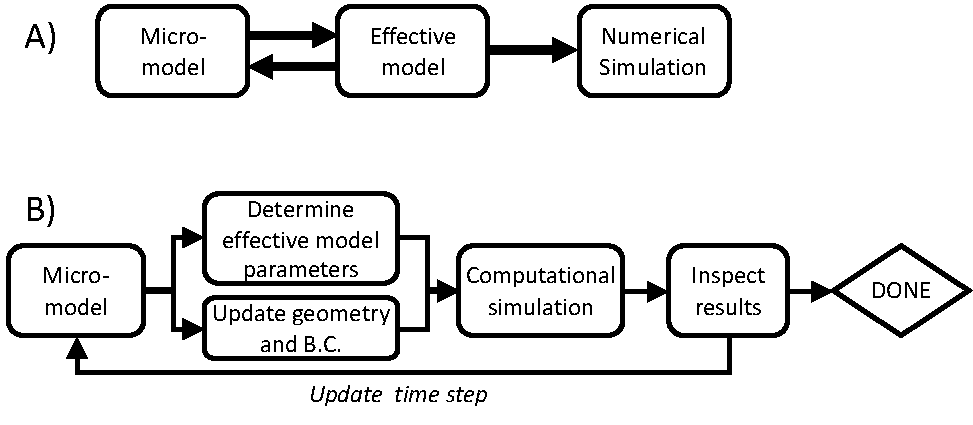
\includegraphics[width=\textwidth]{Images/chapter5/simulationframework}
\caption{Proposed framework for using an effective constitutive model to improve the efficiency of using complex meso- or multi-scale models (micro\Hyphdash models) in numerical simulations. Here, A) effective constitutive models act as an intermediate step between micro-models and numerical simulations, where micro-models inform the changes to the effective constitutive model while the effective constitutive model for the simulation. B) An example of how this may be implemented for time\Hyphdash evolving is shown.}
\label{fig:simulationframework}
\end{figure}
%-------------------     end FIGURE     -------------------%
%%%%%%%%%%%%%%%%%%%%%%%%%%%%%%%%%%%%%%%%%%%%%%%%%%%%%%%%%%%%
    
    
    
    
    
    
    
    


%---    METHODS
%%%%%%%%%%%%%%%%%%%%%%%%%%%%%%%%%%%%%%%%%%%%%%%%%%%%%%%%%%%%%
%%	Constitutive model form									%
%%%%%%%%%%%%%%%%%%%%%%%%%%%%%%%%%%%%%%%%%%%%%%%%%%%%%%%%%%%%%

\section{Effective constitutive model formulation}

%-----------------------------------------------------------
%	Kinematics
%-----------------------------------------------------------
\subsection{Kinematic considerations}
	
	The choice of kinematic basis is the first step to formulate constitutive models. Very often, it is useful to limit the choice of kinematic basis based on the available mechanical data or how well each basis match the response of the soft tissues, thus simplifying the form of the constitutive model and reducing parameter covariance during parameter estimation. However, for our approach, our aim is a highly generalized constitutive model that can match a wide range of possible micro-model responses using the same form, not restricting itself to the response and physics of specific soft tissue types. There is also no limitations to having sufficient mechanical data for parameter estimation, as this will be generated from the micro-models. As such, our considerations for choosing the kinematic basis are mainly:
\begin{enumerate}
    \item Most generalized form for reproducing a wide range of mechanical responses
    \item Simplest form for implementation and computational cost in numerical simulations
    \item Minimal number of parameters
    \item Minimal parameter covariance for parameter estimation
\end{enumerate}
    The smallest set of kinematic variables that can describe a wide range of soft tissues and deformations using the same simple form is ideal. 

    The invariants and pseudo-invariants of the right or left Cauchy Green tensor is very popular for the constitutive models of soft tissues. Indeed, we use them often with our structural models \cite{fata_insights_2014, zhang_meso_2016, Avazmohammadi2017b, sacks_novel_2016, zhang_modeling_2017}. There is a large number of invariants, each describes a facet of deformation: isotropic, volumetric strain, anisotropic, or interactions between them. The breadth of choices allow for more freedom in selecting a best combination when modeling specific soft tissues. However, there are simply too many invariants, and many of which are highly covariant. This does not lend itself for minimizing the number of parameters and the parameter covariance in a single fully generalized form. 
    
    
    It's here that using the components of the strain tensors is more practical for our approach. Although all strains are equivalent for constitutive modeling because they can be expressed with respect to each other, different strain tensors can have different effects when used directly in place of each other in the same form. For us, with the purpose of keeping the constitutive model form simple for implementation, the Green Lagrange strains are the most practical. Based on preliminary testing (Appendix \ref{sec:greenvshencky}), the Green Lagrange strains result in the simplest 2nd Piola Kirchhoff stress and elasticity tensor forms, and have behaviors in that closely matches the response of collagen fibers in soft tissues when under compression. We examined these aspects more closely in Appendix \ref{sec:greenvshencky}. 
    
    It is also convenient to express the Green Lagrange strain tensor with respect to the material axis (Fig. \ref{fig:greenkinematics}), $\mathbf{m}_0$, where
\begin{equation} \label{eqn:greenstrain}
E_m = \mathbf{m}_0\cdot\mathbf{E}\mathbf{m}_0, \quad E_n = \mathbf{n}_0\cdot\mathbf{E}\mathbf{n}_0, \quad E_{\phi} = \mathbf{m}_0\cdot\mathbf{E}\mathbf{n}_0,
\end{equation} 
    and $\mathbf{n}_0$ is the direction orthogonal to $\mathbf{m}_0$ (Fig. \ref{fig:greenkinematics}). This symmetry is helpful for further reducing the constitutive model form. 


%%%%%%%%%%%%%%%%%%%%%%%%%%%%%%%%%%%%%%%%%%%%%%%%%%%%%%%%%%%%
%-------------------	begin FIGURE 	-------------------%
\begin{figure}
\centering
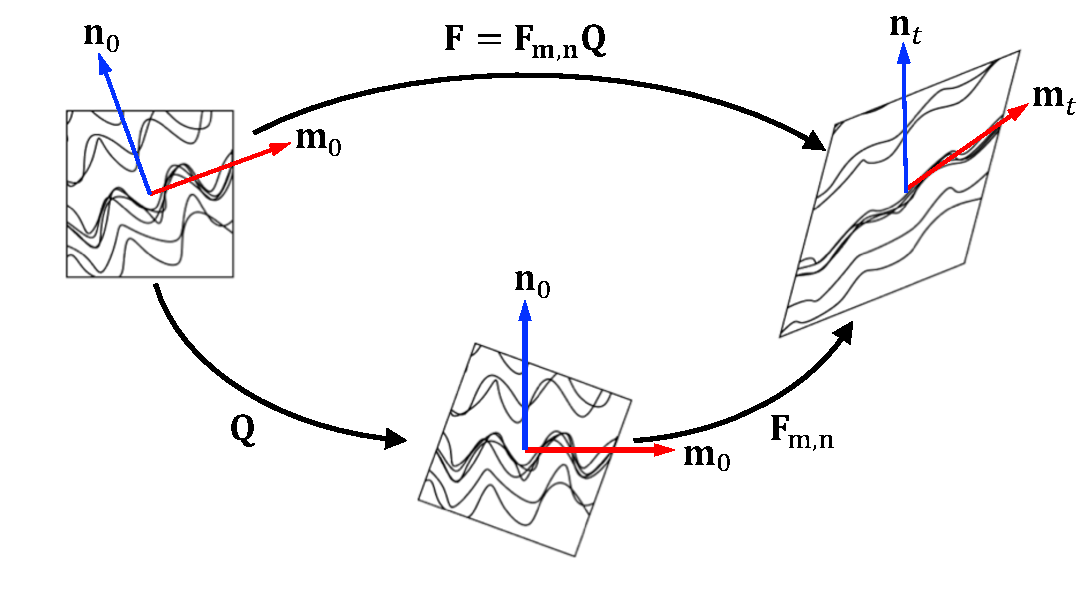
\includegraphics[width=5.0in]{Images/chapter5/greenkinematics.pdf}
\caption{By taking the right polar decomposition of the deformation gradient tensor, we can express the components of the Green Lagrange strain tensor with respect to the material axis. This creates a symmetry for the shear component of the Green Lagrange strain tensor, allowing us to further simplify the model form.}
\label{fig:greenkinematics}
\end{figure}
%-------------------	 end FIGURE 	-------------------%
%%%%%%%%%%%%%%%%%%%%%%%%%%%%%%%%%%%%%%%%%%%%%%%%%%%%%%%%%%%%












%-----------------------------------------------------------
%	Model formulation
%-----------------------------------------------------------
\subsection{Effective constitutive model form}
\subsubsection{Possible family of forms for the effective constitutive model}

    Using phenomenological approaches is necessary for minimal computational cost. The form of phenomenogical models for soft tissues generally falls into three families. The first family is composed of a summation of polynomials, 
%==========================================================%
%-------------------	begin EQUATION 	-------------------%
\begin{equation}
\begin{aligned}
\Psi	&= \sum_i\sum_j\sum_k c_{ijk}E_m^i E_n^j E_\phi^k. 
\end{aligned} \label{eqn:polynomialmodelform}
\end{equation}
%-------------------	 end EQUATION 	-------------------%
%==========================================================%
    We will refer to this family as the polynomial series approach. The second family is composed of separated exponential functions of individual or combinations of invariants or strains used, for example by Vito \textit{et al.} \cite{vito_mechanical_1980},
%==========================================================%
%-------------------	begin EQUATION 	-------------------%
\begin{align}\label{eqn:vitomodelforms}
\Psi 	&= \sum_i\sum_j\sum_k c_{ijk} e^{b_{ijk}E_m^i E_n^j E_\phi^k}.
\end{align}
%-------------------	 end EQUATION 	-------------------%
%==========================================================%
    We will refer to this family as the separated exponential approach. The final family is exponential models composed of a single exponential function of the sum of polynomials,
%==========================================================%
%-------------------	begin EQUATION 	-------------------%
\begin{equation}
\begin{aligned}\label{eqn:exponentialmodelform}
\Psi 	&= c_0 \left(e^{Q} - 1\right) \\
Q		&= \sum_i\sum_j\sum_k b_{ijk}E_m^i E_n^j E_\phi^k.
\end{aligned}
\end{equation}
%-------------------	 end EQUATION 	-------------------%
%==========================================================%
    This was first introduce by Fung \cite{fung_pseudoelasticity_1979} and we will refer to this family as the single exponential approach. 


\subsubsection{Generalized effective constitutive model form determination} \label{sec:possibleforms}

	Each approach (Eqn. \ref{eqn:polynomialmodelform}-\ref{eqn:exponentialmodelform}) has its own advantages and disadvantages. Polynomial series approach has the most flexibility. With sufficient number of terms, it can it reproduce the response in a similar manner to Taylor series expansions. In pilot testing, polynomial series approach requires significantly more number of terms than other choices, at least 27 terms in preliminary testing. 21 of the 27 terms are coupling terms. As a result, constraints needed for convexity are both complex and difficult to enforce. In the most general form, convexity cannot be enforce globally or only at the boundaries. It needs to be enforced at separate points within the domain or by integration. These constraints do not only have computational costs that vastly exceed the cost of the model itself, but will also significantly impacts convergence during parameter estimation. The constraints are not convex, with many local minima, often failing to converge even after 200,000 iterations. In additional, extrapolation using this approach is extremely unreliable. This makes constrained optimization often intractable to implement within a simulation framework such as the one proposed (Fig. \ref{fig:simulationframework}).


	The separated exponential approach generally suffers from the same issues as the polynomial series. This model form behaves like polynomial series with variable exponents, i.e. $c_1e^{b_1E_m} = c_1y^{b_1}$, where $y =e^{E_m}$. The advantage of this family of models is that similar and highly covariant terms such as $c_1 E_m + c_2 E_m^2 + c_3 E_m^3 ...$ can be avoided, reducing the number of parameters needed. However, like the polynomial series family, coupling terms such as $c_4 e^{b_4 E_m E_n}$ are not convex or elliptical functions, resulting in the same issues for parameter estimation and enforcing convexity. The number of parameters required to fully reproduce the mechanical response is still quite large. Moreover, for the same number of parameters, the separated exponential form is woefully insufficient at reproducing the mechanical response of soft tissues in comparison to the single exponential approach. As such, the advantages gained for parameter covariance by separating the terms are actually quite minimal.
    
    The single exponential approach has substantial parameter covariance, but is extremely effective at reproducing the response of soft tissues using a small number of parameters, is computationally efficient, and is easy to enforce convexity for. Because the exponential function is monotonically increasing, enforcing convexity and ellipticity only requires the polynomial $Q$ to be convex and elliptical. This is the best balance for our goals, and is thus our choice for the effective constitutive model. The first step is of course to examine the generalized Fung model \cite{fung_pseudoelasticity_1979}
%==========================================================%
%-------------------	begin EQUATION 	-------------------%
\begin{equation}
\begin{aligned}\label{eqn:fungmodel}
\Psi 	&= c_0 \left(e^{Q} - 1\right) \\
Q		&= \sum_i\sum_j\sum_k\sum_l b_{ijkl}E_{ij} E_{kl}.
\end{aligned}
\end{equation}
%-------------------	 end EQUATION 	-------------------%
%==========================================================%
    We find that the generalized Fung model is not able to fully reproduce the mechanical response of pericardium and aortic valve tissues, it can only do so in a limited range. Although this is enough for most numerical simulations, where the deformations are generally limited to the physiologic range, it is not always sufficient for predicting the mechanical response when organs undergo significant changes in geometry, causing the deformations to change drastically. The easiest way to visualize this is through contour plots of the strain energy function (Fig. \ref{fig:strainenergycontours}). The mechanical response of soft tissues general has hyperelliptical contours (Fig. \ref{fig:strainenergycontours}A), whereas the generalized Fung model always has precisely elliptical contours (Fig. \ref{fig:strainenergycontours}B). This attribute of the generalized Fung model makes it easy to enforce ellipticity and convexity, and its elasticity tensor and behavior at small strains is easy to derive. However, when the range of deformation is sufficiently large, the generalized Fung model is essentially limited to stretching and rotating its contours to match that of the soft tissue (Fig. \ref{fig:strainenergycontours}B), but cannot fully reproduce the resulting tissue responses. It can only serve as an approximation.  


%%%%%%%%%%%%%%%%%%%%%%%%%%%%%%%%%%%%%%%%%%%%%%%%%%%%%%%%%%%%
%-------------------	begin FIGURE 	-------------------%
\begin{figure}
\centering
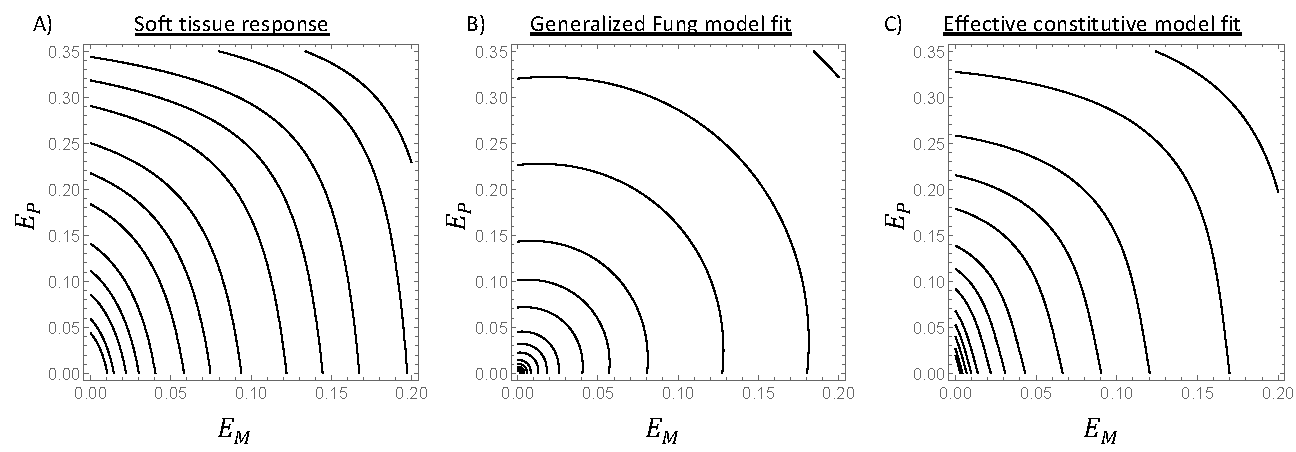
\includegraphics[width=\textwidth]{Images/chapter5/strainenergycontours}
\caption{The contour plots of strain energy (kPa) of A) a bovine pericardial specimen using a meso-scale structural model \cite{zhang_modeling_2017}, B) best fit using the generalized Fung model (Eqn. \ref{eqn:generalizedfungmodel}), and C) best fit using the effective constitutive model we develop from herein showing the necessity of extending existence phenomenological model form.}
\label{fig:strainenergycontours}
\end{figure}
%-------------------	 end FIGURE 	-------------------%
%%%%%%%%%%%%%%%%%%%%%%%%%%%%%%%%%%%%%%%%%%%%%%%%%%%%%%%%%%%%

\subsubsection{Final effective material model form} \label{sec:finalform}

	Thus, for the effective constitutive model, we extended the polynomial $Q$ one step further, allowing hyperellipticity of the strain energy density function (Fig. \ref{fig:strainenergycontours}C). For the additional terms to include, we move up to the next even powers, up to the quartic terms (exponents $i+j+k\leq4$) (Eqn. \ref{eqn:exponentialmodelform}), as odd numbered powers alone do not yield elliptical functions. There are a total of 34 possible terms in Q. Not all terms are required or even admissible. Specifically, the following constraints are enforced on the model:
      
    \underline{Constraint 1}: \underline{The stress must be zero in the reference configuration}. Given that the stress is the gradient of $\Psi$, where is $\Psi^\prime = c_0 Q^\prime e^Q$, all terms in $Q^\prime$ must be zero at zero strain. This corresponds to all $i+j+k = 1$ terms being removed, leaving 31 terms remaining. 
      
    \underline{Constraint 2}: \underline{The response must be elliptic}. That is the shortest line inscribed on the strain energy function surface joining any two points must have a positive curvature. Keeping in mind that the generalized Fung model (Eqn. \ref{eqn:exponentialmodelform}) is already close to being sufficient at reproducing the response of many soft tissues we tested. We only want to extend this to be able to reproduce a wider range of soft tissue responses. Furthermore, in considerations of limiting the number of parameters, reducing parameter correlation, improving the conditioning of the constrained objective function surface, and that the non-elliptical terms must be small, we choose to forgo all $i+j+k = 3$ terms, leaving 21 terms remaining. 
      
    \underline{Constraint 3}: \underline{Response must be independent of the direction of shear}. Since we decompose the Green-Lagrange strain relative to the material axis, this creates a plane of symmetry in the soft tissue response for the direction of shear. Thus, the value of $E_\phi$ can only have even powers, $k = 2,4$. The following terms are thus necessarily zero: $E_m^3E_\phi$, $E_m^2E_nE_\phi$, $E_mE_n^2E_\phi$, $E_n^3E_\phi$, $E_mE_\phi^3$, $E_nE_\phi^3$, $E_mE_\phi$, and $E_nE_\phi$. 
      
The final form of the effective constitutive model is thus
%==========================================================%
%-------------------	begin EQUATION 	-------------------%
\begin{equation}
\begin{aligned}\label{eqn:generalizeexponentialform}
\Psi	=& c_0 \left(e^{Q} - 1\right) \\
Q		=& b_1 E_m^2 + b_2 E_n^2 + b_3 E_\phi^2 + b_4 E_m E_n + b_5 E_m^4 + b_6 E_n^4 + b_7 E_m^3 E_n + b_8 E_m^2 E_n^2 + b_9 E_m E_n^3	\\
	&+ b_{10} E_\phi^4 + b_{11} E_m^2E_\phi^2 + b_{12} E_n^2 E_\phi^2 + b_{13} E_m E_n E_\phi^2.
\end{aligned}
\end{equation}
%-------------------	 end EQUATION 	-------------------%
%==========================================================%








%-----------------------------------------------------------
%	Model convexity
%-----------------------------------------------------------
\subsubsection{Enforcing convexity and ellipticity}

	Perhaps the biggest advantage of the single exponential approach models is the convenience for enforcing ellipticity and convexity. Because ellipticity and convexity are preserved by monotonically increase functions, such as $e^x$, we only have to enforce ellipticity and convexity of $Q$ (Eqn. \ref{eqn:generalizeexponentialform}). For strong ellipticity, the following must be satisfied,
%==========================================================%
%-------------------	begin EQUATION 	-------------------%
\begin{equation}\label{eqn:strongellipticity}
\dmd{\Psi}{2}{F_{ij}}{}{F_{kl}}{}\lambda_i\lambda_k\mu_j\mu_l > 0 \equiv \dmd{Q}{2}{F_{ij}}{}{F_{kl}}{}\lambda_i\lambda_k\mu_j\mu_l > 0,
\end{equation}
%-------------------	 end EQUATION 	-------------------%
%==========================================================%	
	where $F$ is any tensor, and $\lambda$ and $\mu$ are arbitrary non-zero vectors. \emph{This condition is also equivalent of strict convexity \cite{ball_strict_1980}}, so both conditions will be satisfied. Satisfying this constraint requires that the elasticity tensor $C_{ijkl}=\dmd{\Psi}{2}{E_{ij}}{}{E_{kl}}{}$ is positive definite, or rather $\dmd{Q}{2}{E_{ij}}{}{E_{kl}}{}$ is positive definite, satisfying Drucker stability for numerical purposes. Sylvester's criterion \cite{gilbert_positive_1991}, is the most convenient in this scenario, which is given by 
%==========================================================%
%-------------------	begin EQUATION 	-------------------%
\begin{equation}\label{eqn:convexitycriteria}
\begin{aligned}
\dpd[2]{Q}{E_m} \geq 0, \quad
\det
\begin{bmatrix}
\dpd[2]{Q}{E_m} & \dmd{Q}{2}{E_m}{}{E_n}{}\\
\dmd{Q}{2}{E_m}{}{E_n}{} & \dpd[2]{Q}{E_n}\\
\end{bmatrix} \geq0, \quad
\det
\begin{bmatrix}
\dpd[2]{Q}{E_m} & \dmd{Q}{2}{E_m}{}{E_n}{} & \dmd{Q}{2}{E_m}{}{E_\phi}{}\\
\dmd{Q}{2}{E_m}{}{E_n}{} & \dpd[2]{Q}{E_n} & \dmd{Q}{2}{E_n}{}{E_\phi}{}\\
\dmd{Q}{2}{E_m}{}{E_\phi}{} & \dmd{Q}{2}{E_n}{}{E_\phi}{} & \dpd[2]{Q}{E_\phi} \\
\end{bmatrix} \geq0.
\end{aligned}
\end{equation}
%-------------------	 end EQUATION 	-------------------%
%==========================================================%
     For the generalized Fung model (Eqn. \ref{eqn:generalizedfungmodel}), $b_1>0$, $b_1b_2-b_4>0$, and $b_3(b_1b_2 - b_4^2) - b_5(b_2b_5 - b_4b_6) - b_6(b_1b_6 - b_4b5)>0$ will enforce convexity everywhere. For equation \ref{eqn:generalizeexponentialform}, this is slightly more complex. The non-convex region starts from a point along the respective axis for each component $E_m$, $E_n$, and $E_\phi$, then spreads out in the shape of a fan as the strain increases depending on which specific coupling terms, such as $E_m^3 E_n$ and $E_m E_n^3$ are present (Fig. \ref{fig:convexitybehavior}). As long as the effective constitutive model is convex on the largest value along the $E_m$, $E_n$, and $E_\phi$ axis respectively, then the effective constitutive model is convex over the entire range. For example, the effective constitutive model is convex if the maximum point on the $E_m$-axis is convex for $E_m^3 E_n$ (Fig. \ref{fig:convexitybehavior}A) or if the maximum point on the $E_n$-axis is convex for $E_m E_n^3$ (Fig. \ref{fig:convexitybehavior}B). Thus, assuming an upper limit of $E_m < 1$, $E_n < 1$, and $E_\phi < 1$, the following constraints on the parameters are sufficient to guarantee convexity and ellipticity,
%==========================================================%
%-------------------	begin EQUATION 	-------------------%
\begin{equation} \label{eqn:effmodelconstraints}
\begin{aligned}
b_1, b_2,b_3,b_5,b_6,b_{10} \geq 0	\\
4(b_1 + 6 b_5) (b_2 + b_8) - (b_4 + 3 b_7)^2 \geq 0		\\
4(b_2 + 6 b_6) (b_1 + b_8) - (b_4 + 3 b_9)^2 \geq 0 	\\
4(b_1 + b_{11}) (b_2 + b_{12}) - (b_{13} + b_4)^2 \geq 0 	\\
b_3+b_{11} \geq 0	\\
b_3+b_{12} \geq 0.	\\
\end{aligned}
\end{equation}
%-------------------	 end EQUATION 	-------------------%
%==========================================================%


%%%%%%%%%%%%%%%%%%%%%%%%%%%%%%%%%%%%%%%%%%%%%%%%%%%%%%%%%%%%
%-------------------	begin FIGURE 	-------------------%
\begin{figure}
\centering
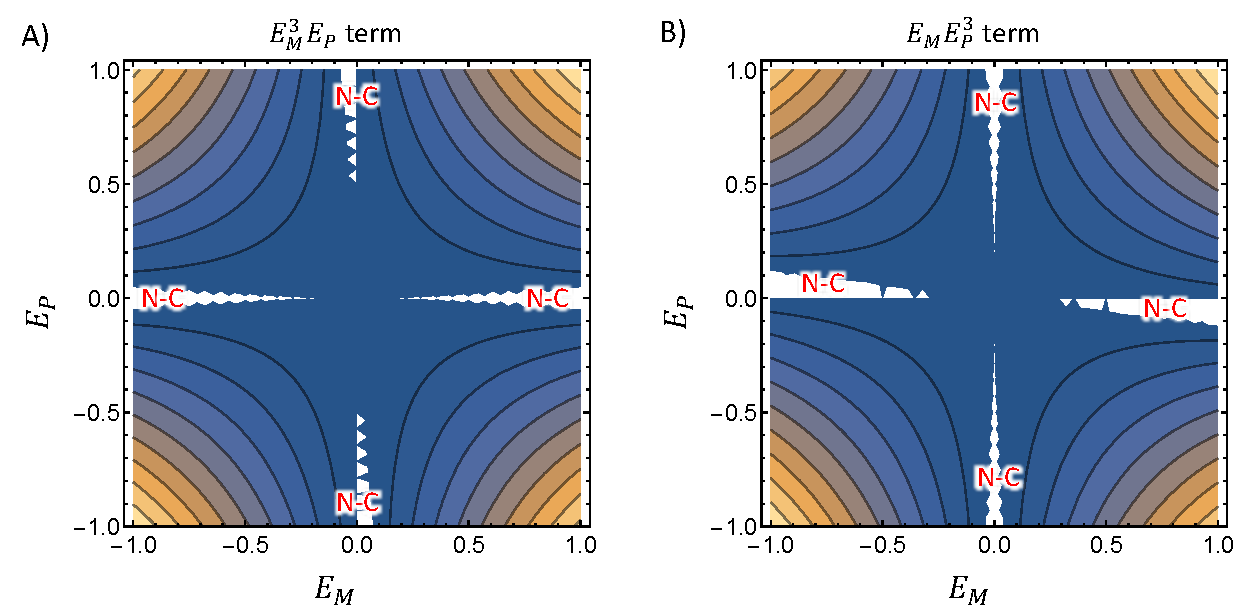
\includegraphics[width=\textwidth]{Images/chapter5/convexitybehavior}
\caption{The criteria for ellipticity (Eqn. \ref{eqn:convexitycriteria}) plotted against the components of the Green-Lagrange strain for A) when including the $E_m^3E_n$ term and B) $E_mE_n^3$ term. The white regions are not convex (N-C), which start at a point along the axes and spreads out as the strain increases.}
\label{fig:convexitybehavior}
\end{figure}
%-------------------	 end FIGURE 	-------------------%
%%%%%%%%%%%%%%%%%%%%%%%%%%%%%%%%%%%%%%%%%%%%%%%%%%%%%%%%%%%%










    
%-----------------------------------------------------------
%	Model scaling for parameter estimation
%-----------------------------------------------------------
\subsection{Model scaling method to improve parameters correlation for parameter estimation} \label{sec:modelscaling}

%-----------------------------------------------------------
%	Computational approaches	
\subsubsection{Parameter correlation for exponential type models}

	One challenging problem with model parameter determination is covariance between the parameters during parameter estimation. Covariance explains how two parameters influence the response of the model and how they will be updated during parameter estimation. High parameter covariance results in both slow convergence and poor reliability and reproducibility of the material parameters. When scaled by the variance, this becomes the correlation between the parameters, with an absolute value between $0$ and $1$. Correlation equal to $1$ implies that two parameters have the exact same effect on the model response, and are thus indistinguishable during parameter estimation. The covariance issue for constitutive models with an exponential function is well described by Aggarwal \cite{aggarwal_inverse_2015, aggarwal_improved_2017}. These constitutive models with exponential functions have a long valley like region in the objective function space. Inside this valley, significantly different parameters produce similar objective function values. This presents several problems. 1) It's difficult to compare model parameters between different specimens, because drastically different parameters can produce similar responses. As such, the average or representative specimen has little real meaning, and each specimen needs to be fitted individually for simulations. 2) The convergence of gradient based optimization algorithms becomes excruciatingly slow due to the small gradients while trapped within this valley. 3) The covariance between parameters being extremely large decreases the accuracy or in other word increases the confidence interval of parameters obtained. 
    
    Aggarwal \textit{et al.} suggested two improvements to alleviate this problem \cite{aggarwal_improved_2017}. These improvements are 1) modifying the modulus parameter $A$ to $e^{a}$, straightening the shape of the valley, and 2) introducing the log-norm for the objective function, improving the gradient along the valley. These modifications have been shown to be effective. However, this is not always ideal. The logarithmic norm suggested faces some issues when fitting stresses or strains, which may be negative and thus becomes undefined. Although this may be alleviated by forgoing data points with negative strains or stresses, but the model may still produce negative values during parameter estimation. Other methods can be used to discard negative values or to take the norm of such values, but these approaches create discontinuities in the gradient of the objective function, causing convergence problems during parameter estimation. Clearly, additional improvements can still be made. 


%-----------------------------------------------------------
%	Scaling method
\subsubsection{Model scaling method}

	We begin by examining the fundamental reason for the high parameter covariance. For this, we will use the 1-D case as an example,
%==========================================================%
%-------------------	begin EQUATION 	-------------------%
\begin{equation}
\begin{aligned}
\Psi &= A \left(e^{B \epsilon} - 1\right) \\
\mathcal{F} &= \sum_i \left(\Psi(\epsilon_i) - \Psi_i \right)^2,
\end{aligned}
\end{equation}
%-------------------	 end EQUATION 	-------------------%
%==========================================================%
where $\Psi$ is the strain energy of our model, $\epsilon$ is some invariant that is a function of the strain, $\epsilon_i$ and $\Psi_i$ are simulated data, and $\mathcal{F}$ is our objective function for parameter estimation. The parameters $A$ and $B$ have different purposes: $A$ is like a modulus, linearly increasing the stiffness of the material, while $B$ modifies the shape of the response, controlling the nonlinearity of the material. However, practically, the two parameters have nearly the same effect on the mechanical response, increasing $A$ increases the stiffness (Fig. \ref{fig:scalingapproach}A) and increasing $B$ also increases the stiffness (Fig. \ref{fig:scalingapproach}B). This is the reason for the high correlation between the parameters (Fig. \ref{fig:scalingapproach}), 0.9979.


%%%%%%%%%%%%%%%%%%%%%%%%%%%%%%%%%%%%%%%%%%%%%%%%%%%%%%%%%%%%
%-------------------	begin FIGURE 	-------------------%
\begin{figure}
\centering
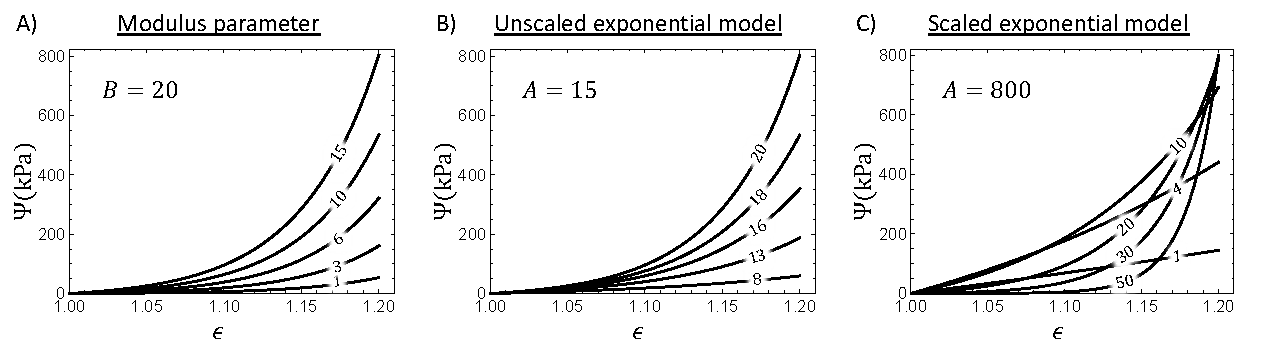
\includegraphics[width=\textwidth]{Images/chapter5/scalingapproach}
\caption{A)The effect of increasing the values of the modulus $A$ on exponential type models. B) The effect of increasing the values of exponent $B$ on exponential type models, which is nearly indistinguishable to the modulus $A$. C) The effect of increasing the values of parameter $B$ after applying the proposed scaling, increasing the values of parameter $A$ remains the same as in A).}
\label{fig:scalingapproach}
\end{figure}
%-------------------	 end FIGURE 	-------------------%
%%%%%%%%%%%%%%%%%%%%%%%%%%%%%%%%%%%%%%%%%%%%%%%%%%%%%%%%%%%%


	To address this problem, we introduce a scaling term to normalize the exponential part of the model, preventing increasing $B$ from increasing the value of the strain energy as a whole, allowing it to only control the curvature. For this, we will use a value $\epsilon_{max}$, which represents the data point with the maximum strain energy value used for parameter estimation, which is also the point where the strain energy stays constant with changes in $B$. The scaled form is thus given by
%==========================================================%
%-------------------	begin EQUATION 	-------------------%
\begin{equation}
\begin{aligned}
\Psi = \Psi_s = \bar{A} \left[e^{-B\epsilon_{max}} \left( e^{B\epsilon} - 1\right)\right],\label{eqn:scaledmodel1D}
\end{aligned}
\end{equation}
%-------------------	 end EQUATION 	-------------------%
%==========================================================%
    where $\bar{A}$ is the scaled version of the modulus $A$. This scaling keeps the exponential part of the model, $e^{-B\epsilon_{max}} ( e^{B\epsilon} - 1)$, at approximately 1.0 at $\epsilon = \epsilon_{max}$, regardless of the changes in the value of the parameter $B$ (Fig. \ref{fig:scalingapproach}C). This effect is not exact when the value of $B$ is small due to the $-1$ needed to set the strain energy to 0 in the referential configuration, but is nonetheless sufficient for our goal: decoupling the modulus increasing effect of the parameter $A$ from the curvature increasing effect of parameter $B$. Indeed, we found this approach to be successful. We examined the contour plot of the objective function with respect to each of the 4 cases in Aggarwal's work \cite{aggarwal_improved_2017}, with the standard objective function, with $A=e^{a}$, with log-norm, and with $A=e^{a}$ and the log-norm, for both without scaling and with scaling (Fig. \ref{fig:objfunctionsurfaces}). First, the correlation between the parameters does not change with $A=e^{a}$. The log-norm improves the correlation from 0.9979 to 0.9063(Table \ref{tb:ABcorrelation}), which significantly improves the objective function surface (Fig. \ref{fig:objfunctionsurfaces}). On the other hand, our scaling method improves the correlation from 0.9979 to 0.6186, more significant than using the log-norm. Interestingly, combining scaling and the log-norm has the adverse effect, increasing the correlation back from 0.6186 to 0.8592. This is a result of essentially linearizing the relation between $A$ and $B$, i.e. from $Ae^{B\epsilon}$ to $Log(A)+B\epsilon$, causing the relationship between $A$ and $B$ to go from modulus and nonlinearity to baseline and modulus. Clearly, \emph{the most optimal parameter estimation approach is to use scaling method with no other modifications}. 
    
    
%%%%%%%%%%%%%%%%%%%%%%%%%%%%%%%%%%%%%%%%%%%%%%%%%%%%%%%%%%%%
%-------------------	begin FIGURE 	-------------------%
\begin{figure}
\centering
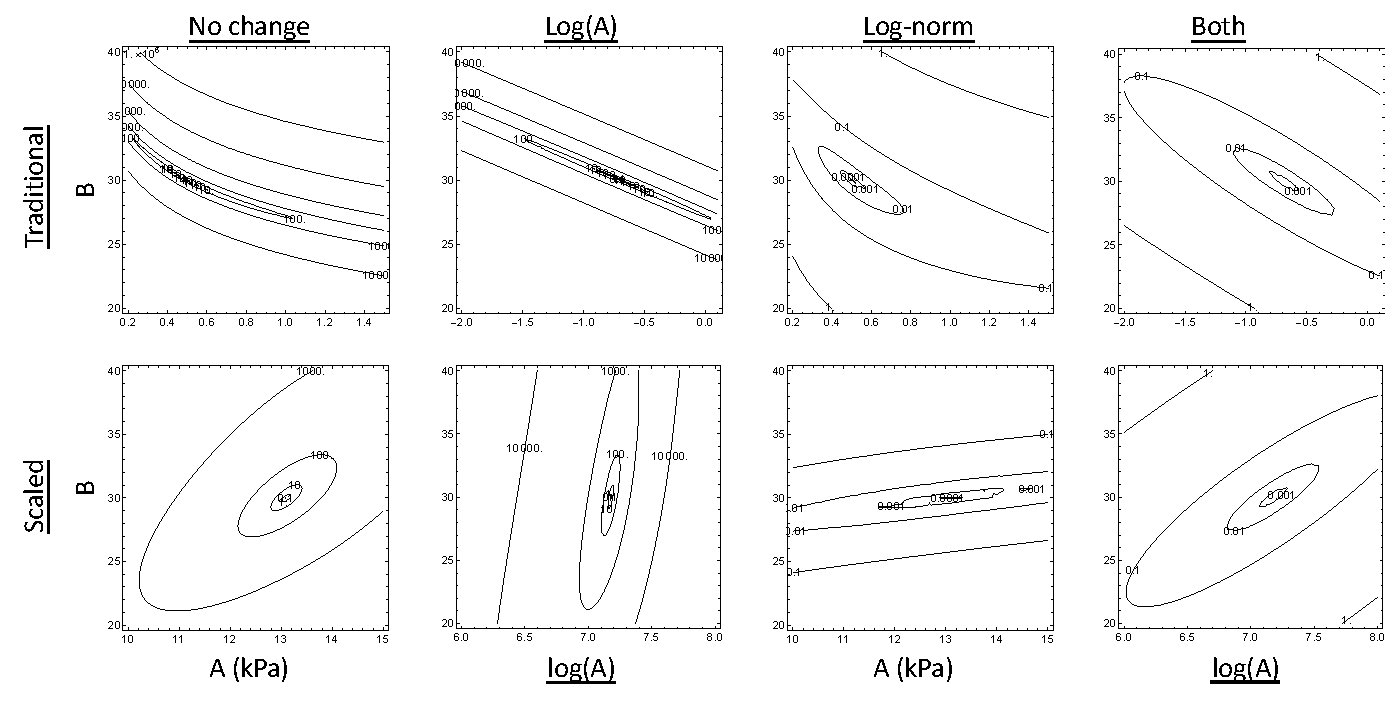
\includegraphics[width=\textwidth]{Images/chapter5/objfunctionsurfaces}
\caption{(Top) The objective function surface for the traditional unscaled exponential models and (Bottom) objective function surface after scaling. From Left to Right are: the unchanged surface, the surface after changing $A$ to $e^{a}$, using the log-norm for the objective function, and applying both changes. The scaled form with no other changes behaves the best.}
\label{fig:objfunctionsurfaces}
\end{figure} 
%-------------------	 end FIGURE 	-------------------%
%%%%%%%%%%%%%%%%%%%%%%%%%%%%%%%%%%%%%%%%%%%%%%%%%%%%%%%%%%%%


%----------------------------------------------------------%
%-------------------	begin TABLE 	-------------------%
\begin{table}
\caption{The correlation between model parameter when using Hencky strains}
\begin{center}
\label{tb:ABcorrelation}
\begin{tabular}{|l|rrrr|}
\hline
			& No change	& $\log(A)$	& $\log$-norm	& Both \\
\hline
Traditional	& -0.9979	& -0.9979	& -0.9063		& -0.9063 \\
Scaled 		& 0.6186	& 0.6186	& 0.8592		& 0.8592 \\
\hline
\end{tabular}
\end{center}
\end{table}
%-------------------	 end TABLE 		-------------------%
%----------------------------------------------------------%



%-----------------------------------------------------------
%	Relation to unscaled form
% \subsubsection{Relation to unscaled model}

    By design, the value of the exponential parameter $B$ does not change by using the scaling method. Since the scaling term does not depend on the input strain, it acts as a modification to the modulus $A$ while keeping the exponential term the same. This also implies that the relationship between the unscaled modulus $A$ and the scaled modulus $\bar{A}$ is
%==========================================================%
%-------------------	begin EQUATION 	-------------------%
\begin{equation}
\begin{aligned}
A = \bar{A} e^{-B\epsilon_{max}},
\end{aligned}
\end{equation}
%-------------------	 end EQUATION 	-------------------%
%==========================================================%
making finding the actual unscaled parameters a simple task. One other benefit of this scaling approach is that the value of $\bar{A}$ is extremely straight forward and intuitive, it is the strain energy of the model at $\epsilon_{max}$. As a result, the value of $\bar{A}$ can be determined \textit{a priori}, or at the very least it is easy to make an initial guess for $\bar{A}$. This will in turn also help to make parameter estimation faster and more accurate, leaving only the parameter $B$ to be determined. 


%-----------------------------------------------------------
%	Extension to multi-variable form
\subsubsection{Extension to multiple variables}

	Extending this method to multiple variables is very simple. For $\Psi_{eff}$ (Eqn. \ref{eqn:finalmodelform}), the input variables become $\mathbf{\epsilon} = \{E_m, E_n, E_\phi\}$, and $\mathbf{\epsilon}_{max} = \{E_m^{max},E_n^{max},E_\phi^{max}\}$. Determining the values for $\mathbf{\epsilon}_{max}$ depends on the form of the objective function. Using the most common case as the example, which is the sum of the squares of the differences in the 2nd Piola Kirchhoff stress,
%==========================================================%
%-------------------	begin EQUATION 	-------------------%
\begin{equation}
\begin{aligned}
\mathcal{F} = \sum_i \left(S_{11}(\epsilon_i) - \hat{S}_{11}^i\right)^2 + \left(S_{12}(\mathbf{\epsilon}_i) - \hat{S}_{12}^i\right)^2 + \left(S_{22}(\epsilon_i) - \hat{S}_{22}^i\right)^2,
\end{aligned}
\end{equation}
%-------------------	 end EQUATION 	-------------------%
%==========================================================%
$\mathbf{\epsilon}_{max}$ is the data point $\mathbf{\epsilon}_i$ which maximizes $\left(\hat{S}_{11}^i\right)^2 + \left(\hat{S}_{12}^i\right)^2 + \left(\hat{S}_{22}^i\right)^2$. 
Thus, we also introduce a $Q_{max}$ such that,
%==========================================================%
%-------------------	begin EQUATION 	-------------------%
\begin{equation} \label{eqn:finalexponentialmodelformscaled}
\begin{aligned}
\Psi_{eff} 	=& c_0 \left(e^{Q} - 1\right) \\
            =& c_0^\prime e^{-Q_{max}}\left(e^{Q} - 1\right)    \\
Q		=& b_1 E_m^2 + b_2 E_n^2 + b_3 E_\phi^2 + b_4 E_m E_n + b_5 E_m^4 + b_6 E_n^4 + b_7 E_m^3 E_n + b_8 E_m^2 E_n^2 + b_9 E_m E_n^3	\\
	&+ b_{10} E_\phi^4 + b_{11} E_m^2E_\phi^2 + b_{12} E_n^2 E_\phi^2 + b_{13} E_m E_n E_\phi^2 \\
Q		=& b_1 (E_m^{max})^2 + b_2 (E_n^{max})^2 + b_3 (E_\phi^{max})^2 + b_4 (E_m^{max}) (E_n^{max}) + b_5 (E_m^{max})^4 + b_6 (E_n^{max})^4   \\ 
    &+ b_7 (E_m^{max})^3 (E_n^{max}) + b_8 (E_m^{max})^2 (E_n^{max})^2 + b_9 (E_m^{max}) (E_n^{max})^3	\\
	&+ b_{10} (E_\phi^{max})^4 + b_{11} (E_m^{max})^2(E_\phi^{max})^2 + b_{12} (E_n^{max})^2 (E_\phi^{max})^2 + b_{13} (E_m^{max}) (E_n^{max}) (E_\phi^{max})^2,
\end{aligned}
\end{equation}
%-------------------	 end EQUATION 	-------------------%
%==========================================================%
where parameter estimation will be done for $c_0^\prime$ instead of $c_0$. Computing the response functions and the stresses, or even the elasticity tensor remains very simple, only requiring multiplying each term by $e^{-Q_{max}}$. Thus, this scaling method is a very simple and easy to implement method of improving the speed and convergence for the parameter estimation of exponential type models. 












%-----------------------------------------------------------
%	Optimal loading paths
%-----------------------------------------------------------
\subsection{Optimal \textit{in silico} loading paths for parameter estimation}\label{sec:optimaldesign}

	Another technique for improving the parameter estimation process for determining $\Psi_{eff}$ from respective micro-models is establishing optimal loading paths. An example is the work of Avazmohammadi \cite{Avazmohammadi2017b}, where optimal experimental design is used to 1) minimize the amount of data necessary and 2) improve model parameter covariance for parameter estimation. Just like one of the most important question to ask before performing any mechanical testing is how much and what kind of data is necessary, we should also be selective with our choice of sampling points for parameter estimation. The theory for optimal design of experiment is well-studied and documented \cite{lanir_optimal_1996, zhu_d_2014}. Vast majority of the methods for optimal design uses D-optimality as the design variable,
%==========================================================%
%-------------------	begin EQUATION 	-------------------%
\begin{equation}\label{eqn:doptimality}
\begin{aligned}
D = \det(\mathbfcal{I}), \quad \mathbfcal{I} = \mathbf{J}^\mathsf{T}\mathbf{J} \quad \mathrm{or} \quad \mathbfcal{I} = \mathbfcal{H},	\\
\mathrm{where} \ J_{ij} = \dpd{f_i}{\xi_j}, \quad \mathcal{H}_{ij} = \dmd{\mathcal{F}}{2}{\xi_i}{}{\xi_j}{},
\end{aligned}
\end{equation}
%-------------------	 end EQUATION 	-------------------%
%==========================================================% 
    where $\mathbf{\xi}$ is a vector of model parameters and $\mathbfcal{I}$ is the information matrix. $\mathbfcal{I}$ can be computed from the derivatives of the objective function $\mathcal{F}$, where $f$ is the model evaluated at each data point, or it can be computed from the Hessian of the objective function, $\mathbfcal{H}$ (Appendix \ref{sec:parametercorrelation}). D-optimality is the determinant of the information or the hessian matrix at the best fit value. It offers the best representation of both parameter accuracy (parameter covariance or correlation) and precision (parameter variance) at the same time.

    
    The first and foremost step is to establish the parameterization for loading paths so they can be optimized. This is not straight a forward choice, as the number of loading path required is not yet established. Another troubling issue is that the number of data points is discrete, thus the gradient of the D-optimality with respect to the control parameters is not smooth. For the sake of time spent for optimization, the number of data points should be kept as small as possible, thus exacerbating the issue of differentiability. Even worse is perhaps that the objective function is essentially flat when not near the optimum, making gradient algorithms not practical. Monte Carlo, random search or divide and conquer strategies are needed, which are much more time consuming. The search space also increases exponentially with the number of loading paths, making a fully exhaustive search difficult to implement. Thus, a simple parameterization for loading paths is ideal. 
    

%%%%%%%%%%%%%%%%%%%%%%%%%%%%%%%%%%%%%%%%%%%%%%%%%%%%%%%%%%%%
%-------------------	begin FIGURE 	-------------------%
\begin{figure}
\centering
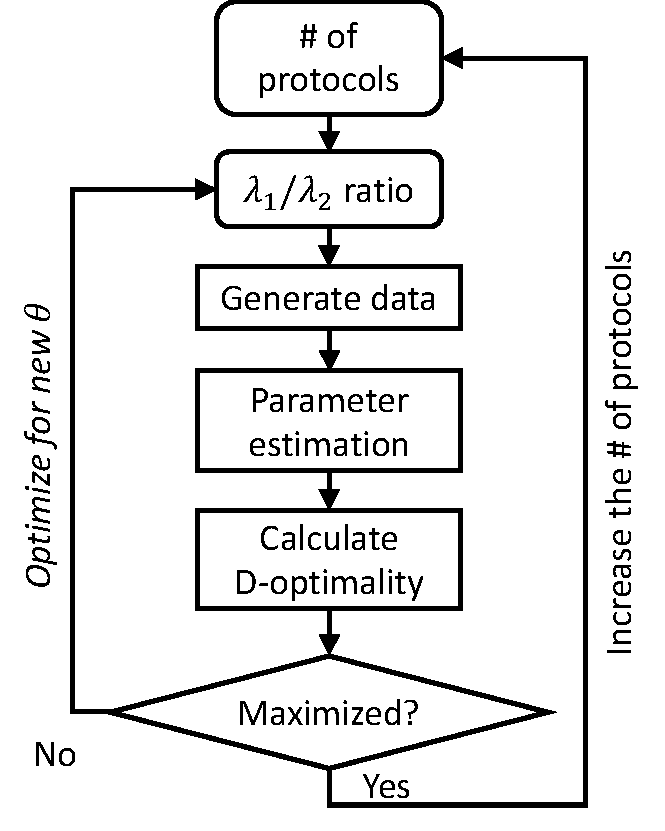
\includegraphics[width=2.5in]{Images/chapter5/optimaldesign}
\caption{Our approach for optimizing for the optimal loading paths for parameter estimation.}
\label{fig:optimaldesign}
\end{figure}
%-------------------	 end FIGURE 	-------------------%
%%%%%%%%%%%%%%%%%%%%%%%%%%%%%%%%%%%%%%%%%%%%%%%%%%%%%%%%%%%%

    
    We define loading paths based on the following conditions: 
\begin{enumerate}
\item The number of loading paths is as small as possible
\item The number of variables needed to define a loading path is as small as possible
\item Possible application to mechanical testing of tissues.
\end{enumerate} 
    Starting with planar extensions only, we chose a loading path as data points which shares the same stretch ratio, $\lambda_1/\lambda_2$, which is typically the same definition used for biaxial mechanical testing. This only requires one constant to be defined for each loading path and the resulting fan shape covers the largest range of deformation with the least number of data points. To determine the optimal loading paths, 1) the total number of loading paths was set, then 2) each combination of the stretch ratios were evaluated for the highst D-optimality (Fig. \ref{fig:optimaldesign}). For a total number of loading paths ranging from 1 to 6, we found the the point when the D-optimality stops increasing significantly, and choose this as the optimal set. Next the shear component, $\kappa_1$, is added. For this study, we constrained the shear to be $0<\kappa_1<0.2$. Only the positive values of $\kappa_1$ is allowed due to the material symmetry. Furthermore, the optimal planar extensions loading paths are always included as a part of the data set.














%%%%%%%%%%%%%%%%%%%%%%%%%%%%%%%%%%%%%%%%%%%%%%%%%%%%%%%%%%%%%
%%  Model Applications										%
%%%%%%%%%%%%%%%%%%%%%%%%%%%%%%%%%%%%%%%%%%%%%%%%%%%%%%%%%%%%%

%-----------------------------------------------------------
%	Use of structural constitutive models
%-----------------------------------------------------------
\subsection{Example application for planar soft tissues}

	The exogenously cross-linked structural model presented in Zhang and Sacks \cite{zhang_modeling_2017} is used to test our approach (Fig. \ref{fig:simulationframework}) and see if $\Psi_{eff}$ (Eqn. \ref{eqn:finalexponentialmodelformscaled}) can completely reproduce its response. This meso-scale structural model is computationally expensive due to integration over the collagen fiber architecture but have been shown to be able to accurately reproduce the mechanical response of a variety of soft tissues, such as mitral valve leaflets \cite{zhang_meso_2016}, ovine pulmonary artery \cite{fata_insights_2014}, myocardium \cite{avazmohammadi_novel_2017}, and exogenously cross-linked bovine pericaridium \cite{sacks_novel_2016}. To briefly summarize, this model is composed of 3 components: collagen, $\Psi_\mathrm{col}$, matrix, $\Psi_\mathrm{mat}$, and interactions, $\Psi_\mathrm{int}$. 
%==========================================================%
%-------------------	begin EQUATION 	-------------------%
\begin{equation}
\Psi 	= \Psi_\mathrm{col} + \Psi_\mathrm{mat} + \Psi_\mathrm{int} \label{eqn:structuralmodelcomponents}
\end{equation}
%-------------------	 end EQUATION 	-------------------%
%==========================================================%
    The matrix term, $\Psi_\mathrm{mat}$, is a modified version of the Yeoh model that is more linear when expressed in 2nd Piola Kirchhoff stress versus stretch, 
%==========================================================%
%-------------------	begin EQUATION 	-------------------%
\begin{equation}\label{eqn:matrixmodel}
\begin{aligned}
\Psi_\mathrm{mat} = &\frac{\eta_M}{2} \left[ \frac{1}{a}\left( I_1 -3\right)^{a} + \frac{r}{b} \left( I_1 -3\right)^{b} \right], \\
&\text{with } 1<a<b, ab <2, 0 \leq r.
\end{aligned}
\end{equation}
%-------------------	 end EQUATION 	-------------------%
%==========================================================%
    This model contains four parameters: $\eta_M$ is the modulus parameter corresponding to the same parameter in the Neo Hookean model, $a$, $b$, and $r$ are the shape parameters, where $a$ and $b$ control the shape of the two terms, while $r$ is the weight between the two terms. In general, $a \approx 1$, $b \approx 1.87$ and $r \approx 15$ can be treated as constants. 


	The response of collagen fibers is given by the integration over the collagen fibers architecture, their orientation and crimp. The fiber orientations is described by a beta distribution function and fiber crimp is described by another beta distribution function of the stretches needed to straighten the fibers, the slack stretch $\lambda_s$. These are referred to as the orientation distribution function (ODF), $\Gamma$, and the recruitment distribution function (RDF), $D$, respectively, with the forms given in Zhang and Sacks \cite{zhang_meso_2016, zhang_modeling_2017, sacks_novel_2016}. The form of the strain energy function is 
%==========================================================%
%-------------------	begin EQUATION 	-------------------%
\begin{equation} \label{eqn:collagen}
\begin{aligned}
\Psi_\mathrm{col} =& \phi_\mathrm{col} \eta_C \int\displaylimits_\theta \Gamma(\theta) 
\int\displaylimits_1^{\lambda_\theta} D\left(\lambda_s \right) \left( \frac{\lambda_\theta}{\lambda_s} - 1\right)^2 \mathrm{d}\lambda_s \mathrm{d}\theta,
\end{aligned}
\end{equation}
%-------------------	 end equation 	-------------------%
%----------------------------------------------------------%
    where $\eta_C$ is the modulus of the collagen fibers, $\lambda_\theta = \sqrt{\mathbf{n}_\theta \cdot \mathbf{C}\mathbf{n}_\theta}$ is the stretch of the ensemble of collagen fiber with the same orientation, and $\lambda_\mathrm{\theta}/\lambda_s$ is the true stretch of the collagen fibers after they are straightened \cite{zhang_meso_2016}. Similarly, the response of the interaction term is given by integration over pairs of fibers based on their orientation and crimp, which contains a quadruple integral. 
%==========================================================%
%-------------------	begin EQUATION 	-------------------%
\begin{equation}
\Psi_\mathrm{int} = \frac{\eta_I}{2} \int\displaylimits_\alpha \int\displaylimits_\beta \Gamma(\alpha) \Gamma(\beta) \int\displaylimits_1^{\lambda_\alpha} \int\displaylimits_1^{\lambda_\beta} D\left( x_\alpha \right) D\left( x_\beta \right) \left( \frac{\lambda_\alpha \lambda_\beta}{x_\alpha x_\beta} - 1\right)^2 \,\mathrm{d}x_\alpha \,\mathrm{d}x_\beta \,\mathrm{d}\alpha \,\mathrm{d}\beta.
\end{equation}
%-------------------	 end EQUATION 	-------------------%
%==========================================================%
For clarity of presentation, the slack stretches, $\lambda_s$, are replaced by $x_\alpha$ and $x_\beta$ for fiber oriented along the angle $\alpha$ and $\beta$ respectively. Only one parameter, the modulus $\eta_I$, is used to account for all interactions, with the same $\Gamma$ and $D$ already given above. 

The second Piola Kirchhoff stress, $\mathbf{S}=2\frac{\partial\Psi}{\partial\mathbf{C}}$, is 
%==========================================================%
%-------------------	begin EQUATION 	-------------------%
\begin{equation} \label{eqn:fullcollagen}
\begin{aligned}
\mathbf{S} = & \phi_\mathrm{col} \eta_C \int\displaylimits_\theta \Gamma(\theta)\left\lbrace 
\int\displaylimits_1^{\lambda_\theta} \frac{D\left( x \right)}{x} \left( \frac{1}{x}- \frac{1}{\lambda_\theta}\right) \mathrm{d}x \right\rbrace \mathbf{n}_\theta\otimes\mathbf{n}_\theta \mathrm{d}\theta \\
+ & \phi_\mathrm{col} \eta_I \int\displaylimits_\alpha \int\displaylimits_\beta \Gamma \left(\alpha \right) \Gamma \left( \beta \right) \\
& \times \left[ \left\lbrace 
\int\displaylimits_1^{\lambda_\alpha} \int\displaylimits_1^{\lambda_\beta} 
\frac{2 \lambda_\beta D(x_\alpha) D(x_\beta)}{x_\alpha x_\beta} 
\left( \frac{\lambda_\alpha}{x_\alpha} \frac{\lambda_\beta}{x_\beta} - 1\right) \mathrm{d}x_\alpha \, \mathrm{d}x_\beta 
+\int\displaylimits_1^{\lambda_\beta} D(x_\beta) \left( \frac{\lambda_\beta}{x_\beta} -1  \right)^2 \mathrm{d}x_\beta \right\rbrace \right.  \frac{\mathbf{n}_\alpha \otimes \mathbf{n}_\alpha}{\lambda_\alpha}  \\
& + \left. \left\lbrace
\int\displaylimits_1^{\lambda_\alpha} \int\displaylimits_1^{\lambda_\beta} 
\frac{2 \lambda_\alpha D(x_\alpha) D(x_\beta)}{x_\alpha x_\beta} 
\left( \frac{\lambda_\alpha}{x_\alpha} \frac{\lambda_\beta}{x_\beta} - 1\right) \mathrm{d}x_\alpha \, \mathrm{d}x_\beta 
+ \int\displaylimits_1^{\lambda_\alpha} D(x_\alpha) \left( \frac{\lambda_\alpha}{x_\alpha} -1  \right)^2 \mathrm{d}x_\alpha \right\rbrace \frac{\mathbf{n}_\beta \otimes \mathbf{n}_\beta}{\lambda_\beta}  \right] \mathrm{d}\alpha \, \mathrm{d}\beta\\
+ & \phi_\mathrm{mat} \eta_M \left[\left(\left( I_1 - 3\right)^{a - 1} + r \left( I_1 - 3\right)^{b - 1}\right) \left( \mathbf{I} - C_{33}\mathbf{C}^{-1}\right)  \right],\\
\end{aligned}
\end{equation}
%-------------------	 end EQUATION 	-------------------%
%==========================================================%
    where $\phi_\mathrm{col}$ and $\phi_\mathrm{mat}$ are the mass fraction of collagen and matrix respectively. 
    
	Although very accurate and predictive, this model is not only computationally expensive, numerical integration also results in a significant decrease in numerical precision when the number of quadrature point is insufficient. This can create a number of issues for convergence during parameter optimization. Thus, the implementation of this model is complicated by a constant balance between computational cost and numerical robustness during optimization. Using $\Psi_{eff}$ to reproduce its response is a solution to these issues. Furthermore, some modifications can be made to reduce the form of $\psi_{eff}$ based on how well each term captures the behavior of the respective material (see Appendix \ref{sec:specificform}).
    
    
    



	









%-----------------------------------------------------------
%	Parameter estimation
%-----------------------------------------------------------
\subsection{Parameter estimation}

	The objective function we use is 
%==========================================================%
%-------------------	begin EQUATION 	-------------------%
\begin{subequations}\label{eqn:objectivefunction}
\begin{gather}
S_m = \dpd{\Psi}{E_m} = \mathbf{m}_0\cdot\mathbf{S}\mathbf{m}_0,
	\quad S_n = \dpd{\Psi}{E_n} = \mathbf{n}_0\cdot\mathbf{S}\mathbf{n}_0,
    \quad S_\phi = \dpd{\Psi}{E_\phi} = 2\mathbf{m}_0\cdot\mathbf{S}\mathbf{n}_0 \label{eqn:responsefunctions}\\
\mathcal{F} = \sum_i^n \left(S_m(\hat{E}_M^i, \hat{E}_S^i, \hat{E}_\phi^i) - \hat{S}_M^i \right)^2 + \left(S_n(\hat{E}_M^i, \hat{E}_S^i, \hat{E}_\phi^i) - \hat{S}_S^i \right)^2 + \left(S_\phi(\hat{E}_M^i, \hat{E}_S^i, \hat{E}_\phi^i) - \hat{S}_\phi^i \right)^2
\end{gather}
\end{subequations}
%-------------------	 end EQUATION 	-------------------%
%==========================================================%
    This removes rigid body rotation and puts the stresses along the material axes, giving the response functions and minimizes covariance between the parameters during optimization. Other possible options include the log of the L2-norm, the log-norm presented by Aggarwal \cite{aggarwal_improved_2017}, and L2-norm of the strain energy and other stresses.


	For optimal speed, gradient methods are ideal. Because we require some non-linear constraints to enforce convexity, we utilized the interior point algorithm provided by the IPOPT library \cite{waechter_implementation_2005}. The initial guess is easily derived for the model scaling method, with the parameter $c_0$ being the maximum strain energy in the available data. The exponent parameters $b_i$ are generally very consistent in value, with the quadratic parameters being $b_1 \approx 10$, $b_2 \approx 10$, and $b_4 \approx -10$, the quartic parameters being $b_5 \approx 2000$, $b_6 \approx 500$, $b_9 \approx 200$, $b_{10} \approx 200$, $b_{11} \approx 200$, $b_{12} \approx 200$. We find this setup to work extremely well, and no further modification being necessary. 




\subsection{Reproducing the response of soft tissues using the effective constitutive model and optimal loading paths}\label{sec:reproducefung}

	For our approach (Fig. \ref{fig:simulationframework}), we need to overcome the limitation of common phenomenological approaches on predicting the mechanical response of micro-models outside of the data set used for parameter estimation \cite{sun_biaxial_2003}. To verify this, we will first reproduced the results of Sun \textit{et al.} \cite{sun_biaxial_2003} using the generalized Fung model, then repeat the process using $\Psi_{eff}$ (Eqn. \ref{eqn:finalexponentialmodelformscaled}) with optimal loading paths. We will focus on glutaraldehyde cross-linked bovine pericardium as the tissue. Bovine pericardium is the most common material used to fabricate bioprosthetic heart valves. It is extremely dense in collagenous fibers, having broad fiber splays with approximately $30\deg$ in standard deviation. The resulting mechanical behavior have strong coupling between the axial stretches. Thus, the mechanical response of some bovine pericardium specimens are fitted to the structural model (Eqn. \ref{eqn:fullcollagen}). The structural model is then used to generate stress strain data along loading paths with stress ratios ($S_{11}/S_{22}$) of $0.1:1$, $0.5:1$, $0.75:1$, $1:1$, $1:0.75$, $1:0.5$, and $1:0.1$. Following Sun \textit{et al.} \cite{sun_biaxial_2003}, the generalized Fung model (Eqn. \ref{eqn:generalizedfungmodela}) was fitted to the five loading paths in the physiologic range ($0.5:1$, $0.75:1$, $1:1$, $1:0.75$, $1:0.5$), then the remain two loading paths were predicted and compared to the data. Next, the reverse scenario was done, where the generalized Fung model was fitted to the non-physiologic loading paths ($0.1:1$ and $1:0.1$), while the remaining five loading paths were predicted. Following the same step, $\Psi_{eff}$ was fitted to the three optimal loading paths ($0.1:1$, $1:1$, and $1:0.1$) while the remaining loading paths were predicted. 
    
    We also considered some alternative loading paths. In the original paper by Fung et al. on the constitutive modeling of arteries \cite{fung_pseudoelasticity_1979}, they discussed the use of 'physiologic protocols' as the optimal data set for parameter estimation. These 'physiologic protocols' are loading paths that cover a range past some predetermined lower bounds for $E_{11}$ and $E_{22}$. Conceptually, this is meant to correspond to the range after accounting for the prestrain between the zero stress configuration and the \textit{in vivo} unloaded (not stress free) configuration. For clarity, to distinguish between this and the physiologic range (the range where the physiologic loading path is likely to reside) in Sun \textit{et al.}, we will refer to this as the prestrained range. We reproduced the prestrained protocols in figure 5 of Fung \textit{et al.} \cite{fung_pseudoelasticity_1979}, and compared the results to those with optimal loading paths. 





\subsection{Numerical simulations}

	An exhaustive numerical study using $\Psi_{eff}$ (Eqn. \ref{eqn:finalexponentialmodelformscaled}) is beyond the scope of this work. However, we hereby present an example implementation of the framework we proposed (Fig. \ref{fig:simulationframework}) using $\Psi_{eff}$ (Eqn. \ref{eqn:finalexponentialmodelformscaled}) to homogenize the structural model (Eqn. \ref{eqn:fullcollagen}) for facilitating numerical simulation of intact bioprothetic heart valves. The leaflet material consider are bovine pericardium (most commonly used for bioprothetic heart valve leaflets), porcine aortic valve (highly anisotropy response), and bovine pericardium with an uniform fiber ODF (isotropic). We replicated the response of these tissues using the structural model based on their microstructure. We then fit $\Psi_{eff}$ to the structural model by sampling along optimal loading paths. Next, we evaluated the computational cost and numerical robustness of $\Psi_{eff}$ and its ability to handle a wide range of material properties and the complex \textit{in vivo} deformations in numerical simulations.
    
    
    For numerical simulation, we utilized the custom finite element simulation software developed by Hsu \textit{et al.} \cite{hsu_dynamic_2015, kamensky_immersogeometric_2015, kiendl_isogeometric_2015, wu_anisotropic_2018}. Briefly, the finite element code was developed for isogeometric fluid solid dynamics simulation of heart valves, focusing mostly on the tri-leaflet atrioventricular valves. The tri-leaflet geometry is based on the commonly used Edwards Pericardial Heart Valve with Kirchhoff-Love shells for the leaflets \cite{kiendl_isogeometric_2015} and finite element solver developed in by Kamensky \textit{et al.} \cite {kamensky_immersogeometric_2015}. We utilized this code to simulate leaflet deformation under physiological quasi--static transvalvular pressure. 
    A total was 484 B\'ezier elements was used for each leaflets, with a leaflet density of 1.0 g/cm$^3$ and a uniform leaflet thickness of 0.386mm thick \cite{hsu_dynamic_2015}. Contact between leaflets is handled by a penalty-based approach and imposed at quadrature points of the shell structure, and clamped boundary condition is applied to the leaflet attachment edge. 
    For simplicity and consistency, the collagen fiber direction was assume to be aligned to the circumferential direction of each leaflet. No root, atrial chamber or the surrounding artery was used. The bioprothetic heart valve stent was made rigid and undeformable, serving a stationary reference for the leaflets. A similar validation process to the one presented by Wu \textit{et al.} \cite{wu_anisotropic_2018} to verify the implementation.


%---    Results
\section{Results}

%%%%%%%%%%%%%%%%%%%%%%%%%%%%%%%%%%%%%%%%%%%%%%%%%%%%%%%%%%%%%
%%  Optimal loading paths for parameter estimation  %%%%%%%%%

\subsection{Optimal \textit{in silico} loading paths for parameter estimation}

	The optimal loading paths for reproducing the response of dense collagenous soft tissues such as bovine pericardium and porcine aortic valve consist of 8 loading paths (Fig. \ref{fig:doptimality}C): 5 loading paths consisting of only inplane extensions (Fig. \ref{fig:doptimality}D), and 3 with the addition of the shear component. The increase in D-optimality is significantly less after three loading paths for the in-plane extensions (Fig. \ref{fig:doptimality}A). Same is true for the loading paths with shear. These three loading paths are the equibiaxial stress (Fig. \ref{fig:doptimality}B, Blue), and two uniaxial loading paths (Black, Green). The type of stress is consistent with the stress used for parameter estimation. The loading paths with shear simply iterates on these three loading paths by adding the shear component, we specified the maximum strain to be applied to be $0.2$. We consider this to be the minimal number of loading paths necessary for parameter estimation. In practice, it's better to add the intermediate inplane tension loading paths (Red, Orange) as a precaution, forming the full set of 8 loading paths (Fig. \ref{fig:doptimality}C). 
	
	
	The equi-biaxial stress loading path is the most important loading path. The D-optimality is $10^{-17}$ for the equi-biaxial loading path versus less than $10^{-300}$ (using \textit{Mathematica}'s extended precision) for other loading paths. The set of optimal loading paths will always contain the equi-biaxial stress loading path if the total number is odd, whereas it will always contain two loading paths just beside the equi-biaxial loading paths if it is even. The other loading paths complement the equi-biaxial loading path by spanning the range being searched. More details on the optimal loading path results are presented in appendix \ref{sec:optimalpaths}.
	
%-------------------	begin FIGURE 	-------------------%
\begin{figure}[hbtp]
\centering
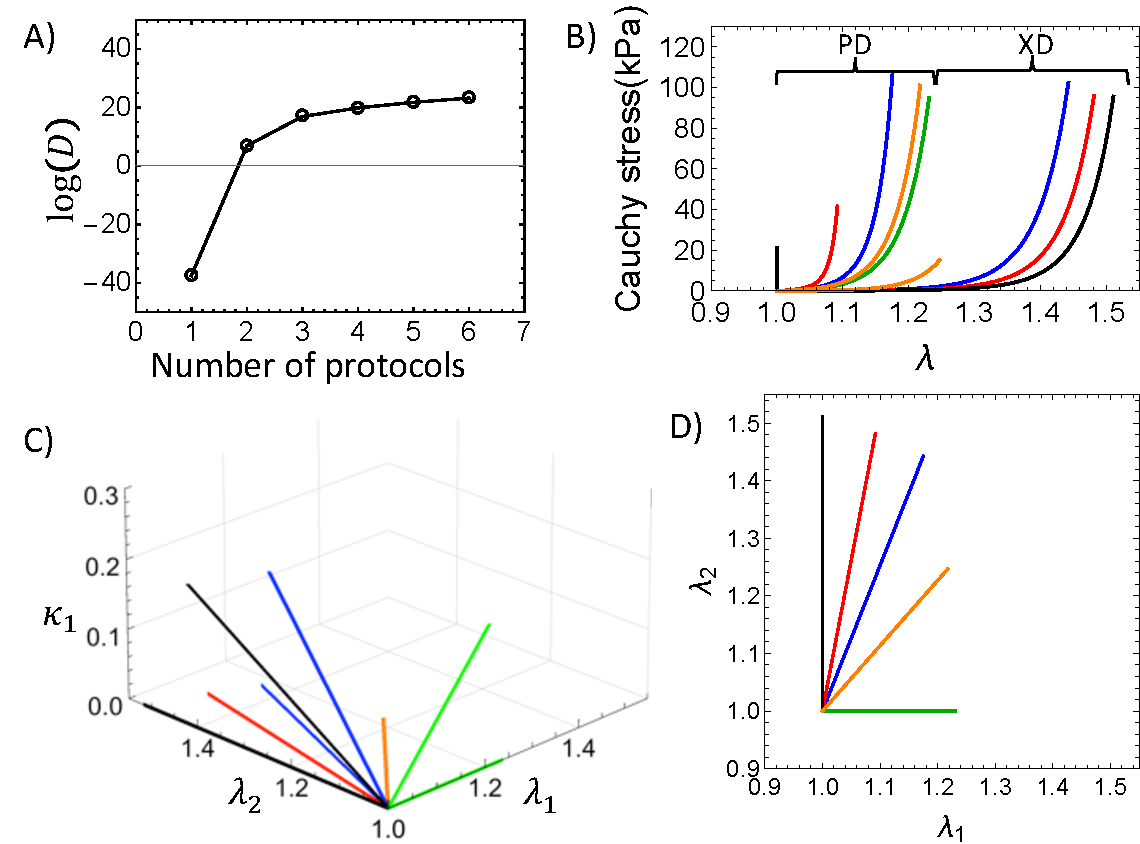
\includegraphics[width=5.5in]{Images/chapter5/doptimality}
\caption{A) The best D-optimality value for a given number of loading paths used to generate the data, which stops increasing significantly after three. B) The stress-strain curve of the optimal set of five loading paths with no shear. C) The full set of optimal loading paths including the shear component are shown. The same colored loading paths are built upon the corresponding D) planar stretch loading paths by adding a shear component. }
\label{fig:doptimality}
\end{figure} 
%-------------------	 end FIGURE 	-------------------%









%%%%%%%%%%%%%%%%%%%%%%%%%%%%%%%%%%%%%%%%%%%%%%%%%%%%%%%%%%%%%
%%  Parameter estimation and the quality of fit             %

\subsection{Parameter estimation and the quality of fit}

    The time taken for parameter estimation (5-10 seconds) is significantly lower in comparison to meso-scale structural approaches, such for the mitral valve \cite{zhang_meso_2016} (10-40 minutes) and exogenously crosslinked tissues \cite{zhang_modeling_2017}(30 min - 4 hours). In addition, we found that the model scaling method significantly improves the consistency of convergence. Parameters converges in approximately 40-60 iterations regardless of starting point, whereas it can vary between 40-120 iterations without using scaling. The additional iterations occur within the valley like region in the objective function surface (Fig. \ref{fig:objfunctionsurfaces}), where the gradient and thus the step size is very small. Of course, we found both methods to be essentially equivalent with a sufficiently good initial guess. We note that the model scaling method does not improve the correlations between the exponent parameters $b_1-b_{13}$ in $Q$. With that being said, the correlations between the exponent parameters $b_1-b_{13}$ are significantly better than the correlations between these exponents and modulus $c_0$ (Fig. \ref{fig:gvsecorrelation} and Appendix \ref{sec:parametercorrelation} Table \ref{tb:correlationE} \& \ref{tb:correlationG} vs. Table \ref{tb:ABcorrelation}), which is not much of a problem for parameter estimation. It is difficult to further improve the parameter correlation of $Q$ without changing the form of the model, but, for our purpose, this is already sufficient. 
    
    
    Qualitatively, $\Psi_{eff}$ (Eqn. \ref{eqn:finalexponentialmodelformscaled}) matches the response of collagenous soft tissues reproduced using the structural model (Eqn. \ref{eqn:fullcollagen}). It is able to follow all the characteristics of the response function (derivatives of the strain energy density function), including the symmetry with respect to shear (Fig. \ref{fig:modelfit}). The average $R^2$ is 0.958 (n = 6) for the bovine pericardium specimens tested. We found similar values for porcine aortic valve leaflets. The main improvements are in the uniaxial strain regions. 
%-------------------	begin FIGURE 	-------------------%
\begin{figure}[hptb]
\centering
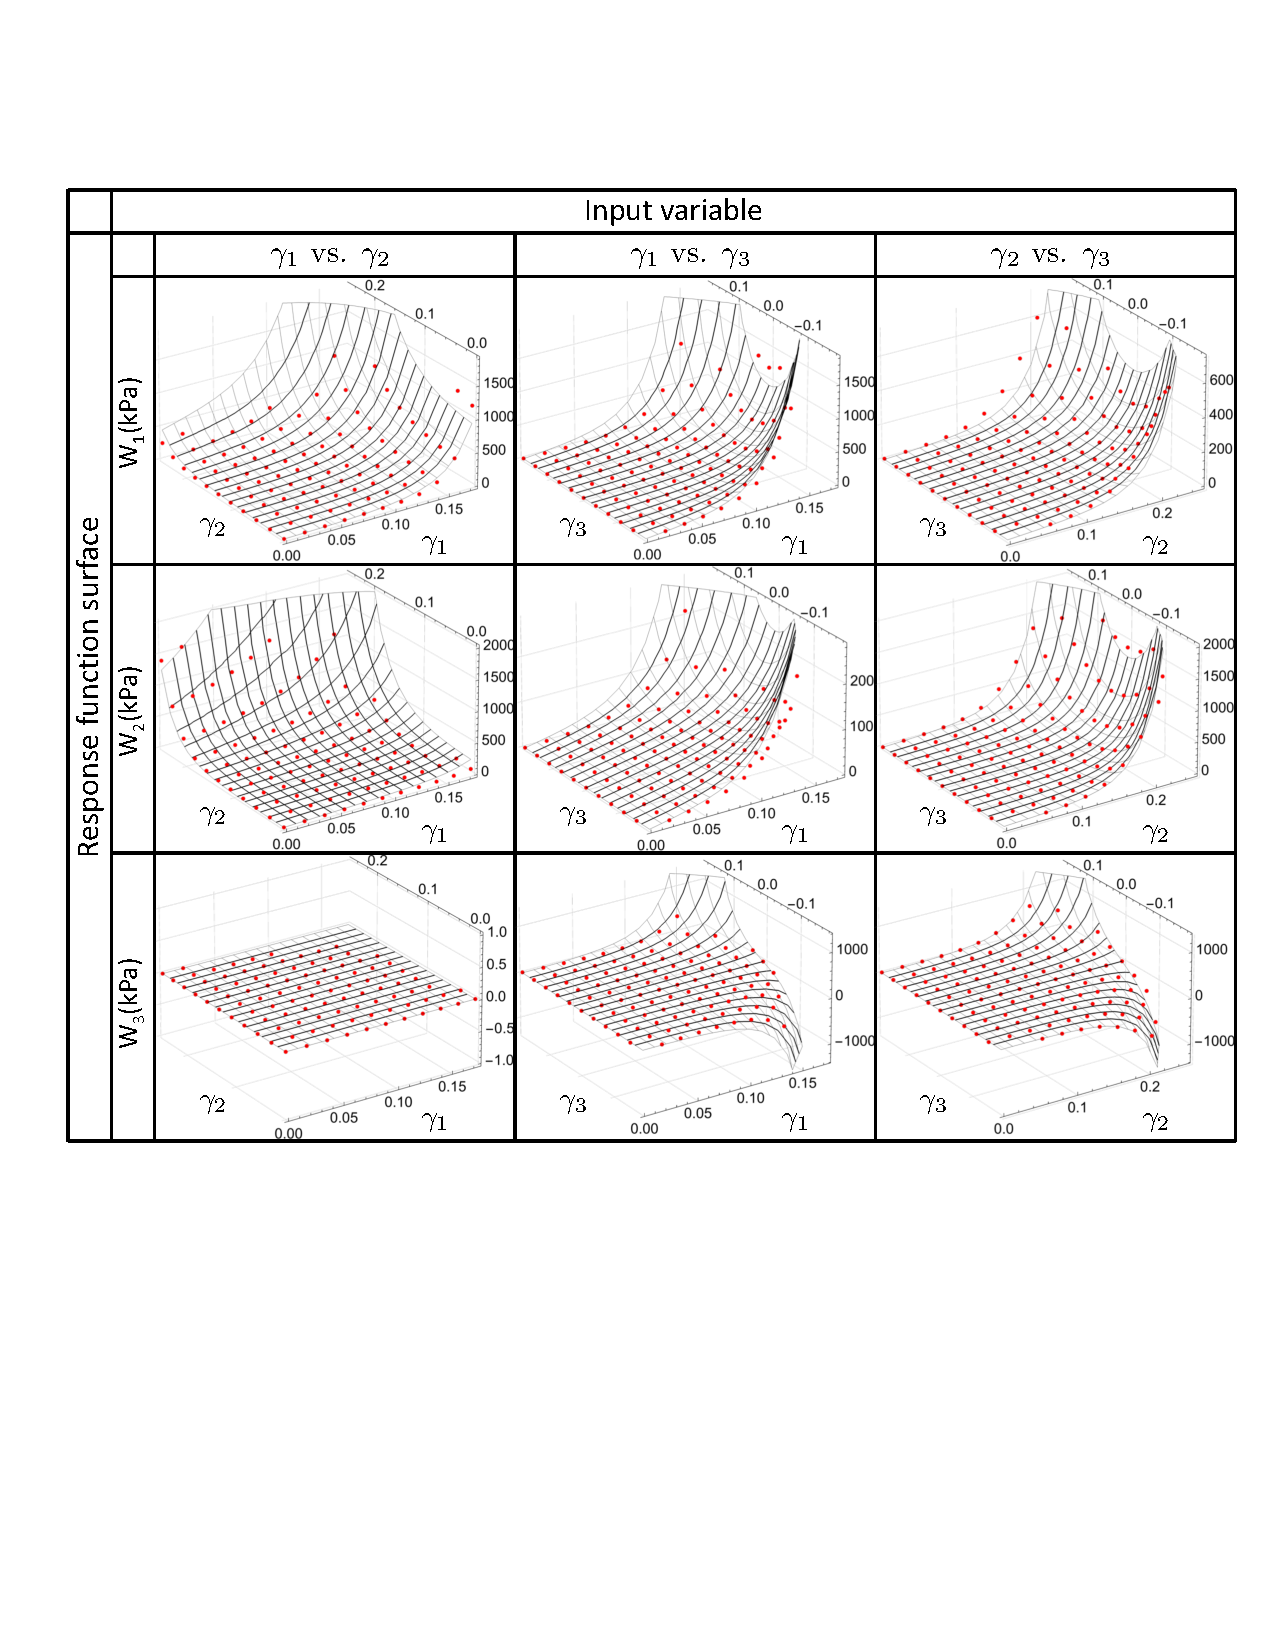
\includegraphics[width=\textwidth]{Images/chapter5/modelfit}
\caption{Parameter estimation results showing that $\Psi_{eff}$ is able to replicate the response function of the structural model (Eqn. \ref{eqn:objectivefunction}) (Top) $S_m = \partial\Psi/\dif E_m$, (Middle) $S_n = \partial\Psi/\dif E_n$, and (Bottom) $S_\phi = \partial\Psi/\dif E_\phi$ for each pair of Green Lagrange strain components.}
\label{fig:modelfit}
\end{figure} 
%-------------------	 end FIGURE 	-------------------%


    For a more detailed comparison, we replicated the result of Sun \textit{et al.} \cite{sun_biaxial_2003}. Similarly, we found that the generalized Fung model (Eqn. \ref{eqn:generalizedfungmodela}) fitted the five loading paths in the physiologic range very well (Fig. \ref{fig:fungphyfit}), but predicted the remaining unfitted loading paths poorly (Fig. \ref{fig:fungphypred}). When the non-physiologic loading paths are fit ((Fig. \ref{fig:fungphyfit})), the remaining protocols are still predicted poorly. However, we do note here that the generalized Fung model cannot fit the non-physiologic protocols very well, illustrating the limitation of the generalized Fung model at fitting the response of soft tissue in a wide range of deformations (Section \ref{sec:possibleforms}). 

%%%%%%%%%%%%%%%%%%%%%%%%%%%%%%%%%%%%%%%%%%%%%%%%%%%%%%%%%%%%
%-------------------	begin FIGURE 	-------------------%
\begin{figure}[hptb]
\centering
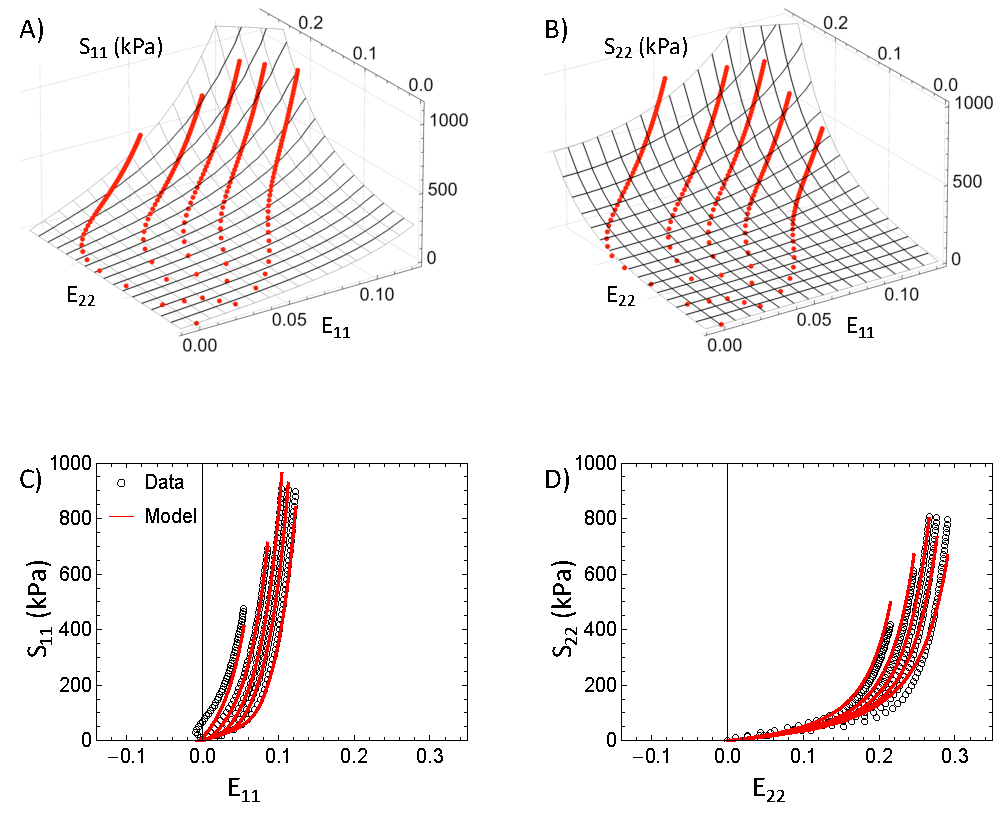
\includegraphics[width=\textwidth]{Images/chapter5/fungphyfit}
\caption{Reproducing the results of Sun \textit{et al.} \cite{sun_biaxial_2003} showing that the generalized Fung model is able to fit the loading paths in the physiologic range very well. A) The $S_{11}$ surface fitted to the data points. B) The $S_{22}$ surface fitted to the data points. C) Best fit of the $S_{11}$ component of the loading paths. D) Best fit of the $S_{22}$ component of the loading paths.}
\label{fig:fungphyfit}
\end{figure} 
%-------------------	 end FIGURE 	-------------------%
%%%%%%%%%%%%%%%%%%%%%%%%%%%%%%%%%%%%%%%%%%%%%%%%%%%%%%%%%%%%

%%%%%%%%%%%%%%%%%%%%%%%%%%%%%%%%%%%%%%%%%%%%%%%%%%%%%%%%%%%%
%-------------------	begin FIGURE 	-------------------%
\begin{figure}[hptb]
\centering
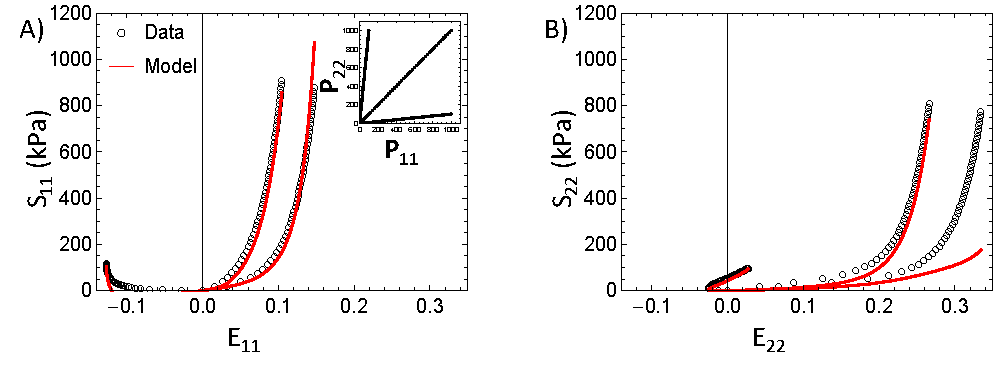
\includegraphics[width=\textwidth]{Images/chapter5/fungphypred}
\caption{Reproducing the results of Sun \textit{et al.} \cite{sun_biaxial_2003} showing the A) $S_{11}$ component and B) $S_{22}$ component of the remaining unfitted loading paths are predicted poorly from fit (Fig. \ref{fig:fungphyfit}). The inset in A shows the corresponding loading paths.}
\label{fig:fungphypred}
\end{figure} 
%-------------------	 end FIGURE 	-------------------%
%%%%%%%%%%%%%%%%%%%%%%%%%%%%%%%%%%%%%%%%%%%%%%%%%%%%%%%%%%%%


%%%%%%%%%%%%%%%%%%%%%%%%%%%%%%%%%%%%%%%%%%%%%%%%%%%%%%%%%%%%
%-------------------	begin FIGURE 	-------------------%
\begin{figure}[hptb]
\centering
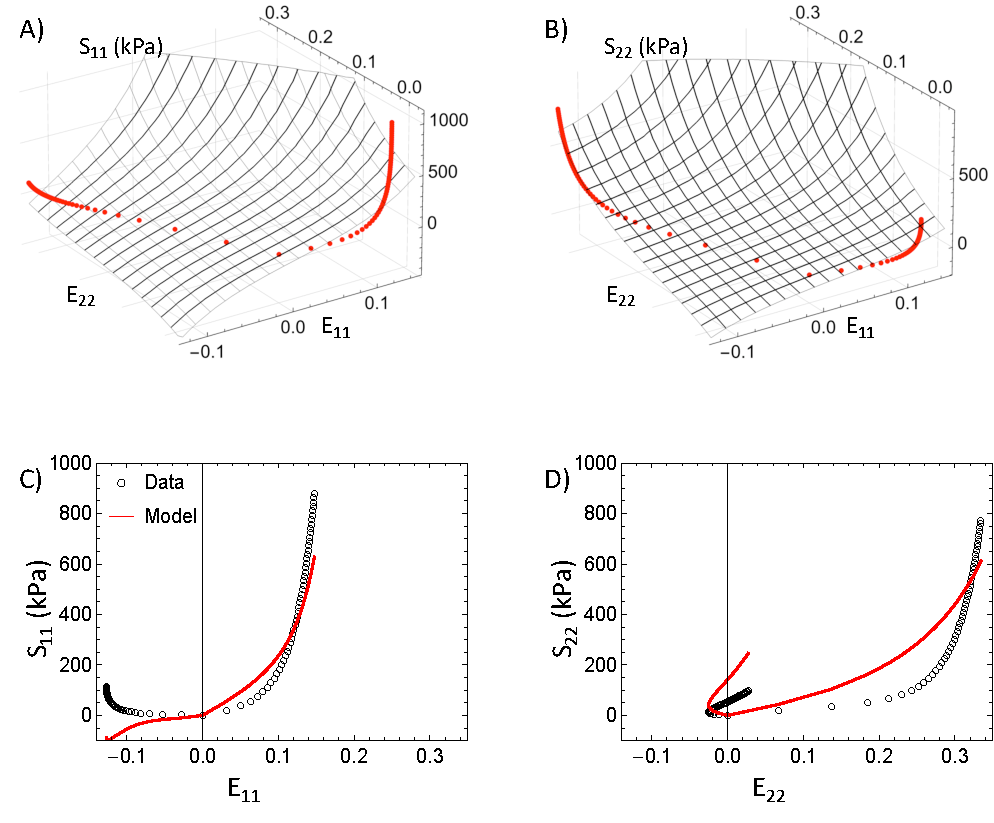
\includegraphics[width=\textwidth]{Images/chapter5/fungoutfit}
\caption{Reproducing the results of Sun \textit{et al.} \cite{sun_biaxial_2003} showing the best fit of the generalized Fung model to the loading paths in the non-physiologic range is poor. A) The $S_{11}$ surface fitted to the data points. B) The $S_{22}$ surface fitted to the data points. C) Best fit of the $S_{11}$ component of the loading paths. D) Best fit of the $S_{22}$ component of the loading paths.}
\label{fig:fungoutfit}
\end{figure} 
%-------------------	 end FIGURE 	-------------------%
%%%%%%%%%%%%%%%%%%%%%%%%%%%%%%%%%%%%%%%%%%%%%%%%%%%%%%%%%%%%

%%%%%%%%%%%%%%%%%%%%%%%%%%%%%%%%%%%%%%%%%%%%%%%%%%%%%%%%%%%%
%-------------------	begin FIGURE 	-------------------%
\begin{figure}[hptb]
\centering
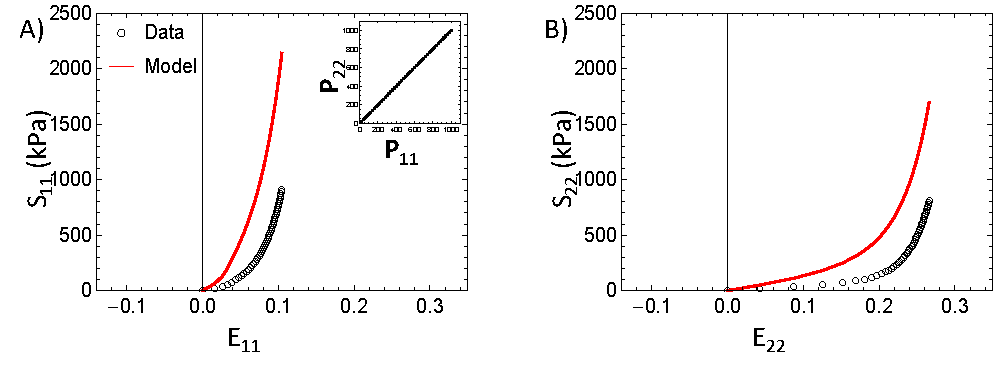
\includegraphics[width=\textwidth]{Images/chapter5/fungoutpred}
\caption{Reproducing the results of Sun \textit{et al.} \cite{sun_biaxial_2003} showing the A) $S_{11}$ component and B) $S_{22}$ component of the equi-biaxial stress loading path are predicted poorly from fit (Fig. \ref{fig:fungoutfit}). The inset in A shows the corresponding loading paths.}
\label{fig:fungoutpred}
\end{figure} 
%-------------------	 end FIGURE 	-------------------%
%%%%%%%%%%%%%%%%%%%%%%%%%%%%%%%%%%%%%%%%%%%%%%%%%%%%%%%%%%%%
    

	Using $\Psi_{eff}$ (Eqn. \ref{eqn:finalexponentialmodelformscaled}) (Fig. \ref{fig:effphyfit}) improves these results, but using non-optimal loading paths, such as based on Fung \textit{et al.}'s prestrained protocols \cite{fung_pseudoelasticity_1979}, lead to poor predictions for other loading paths (Fig. \ref{fig:effphypred}). Although not obvious at first, $\Psi_{eff}$ severely underestimates the response of the material in the low stress region. The D-optimality with two protocols in this prestrained range is only $1.35$, which improves to $1.98\times 10^4$ with six protocols. This pales in comparison to $9.7 \times 10^2$ for the two optimal protocols and $2.2 \times 10^7$ with three optimal protocols. When both $\Psi_{eff}$ and three optimal loading paths are utilized, we found that the loading paths are both fitted (Fig. \ref{fig:effoptfit}) and predicted very well (Fig. \ref{fig:effoptpred}). We also tested other non-optimal loading paths with modifications to the form of $\Psi_{eff}$ (Appendix \ref{sec:otherresults}). To briefly summarize these results, with an optimal set of loading paths, $\Psi_{eff}$ is able to fully reproduce the response of collagenous soft tissue for a wide range of deformation. However, without optimal loading paths, the form of $\Psi_{eff}$ can have unpredictable impact on the predicted response, even though the quality of fit is very similar. 


%%%%%%%%%%%%%%%%%%%%%%%%%%%%%%%%%%%%%%%%%%%%%%%%%%%%%%%%%%%%
%-------------------	begin FIGURE 	-------------------%
\begin{figure}[hptb]
\centering
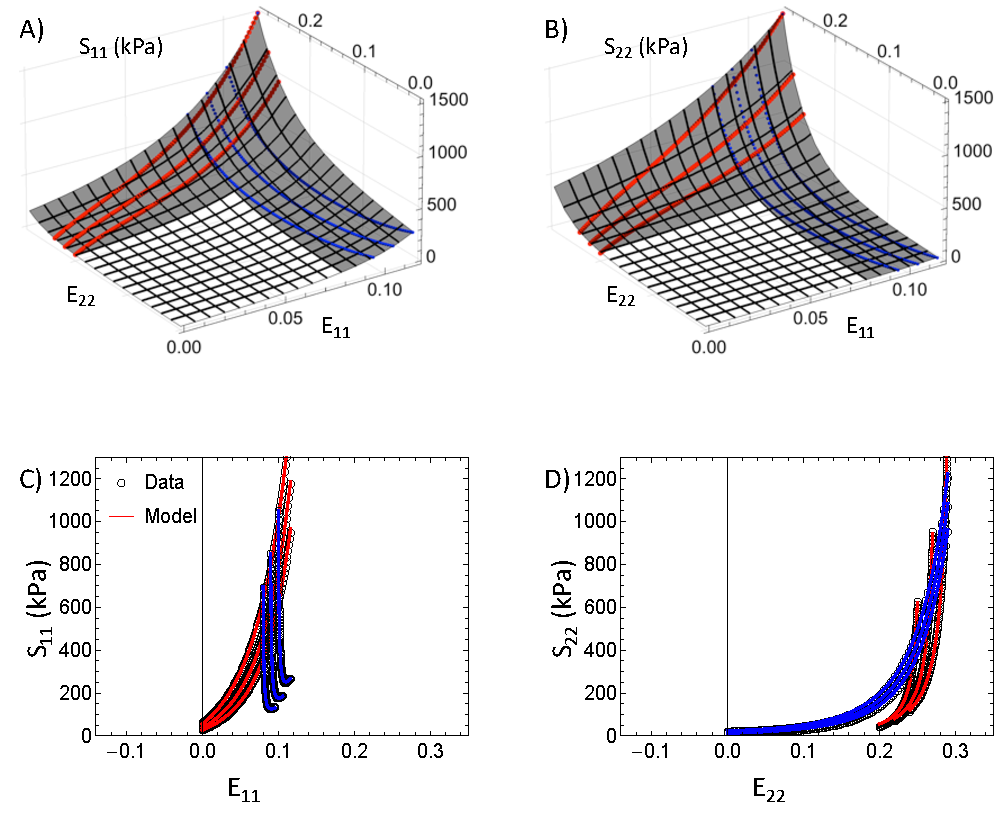
\includegraphics[width=\textwidth]{Images/chapter5/effphyfit}
\caption{The fit of $\Psi_{eff}$ to the prestrained loading paths is very good. A) The $S_{11}$ surface fitted to the data points. B) The $S_{22}$ surface fitted to the data points. C) Best fit of the $S_{11}$ component of the loading paths. D) Best fit of the $S_{22}$ component of the loading paths.}
\label{fig:effphyfit}
\end{figure} 
%-------------------	 end FIGURE 	-------------------%
%%%%%%%%%%%%%%%%%%%%%%%%%%%%%%%%%%%%%%%%%%%%%%%%%%%%%%%%%%%%

%%%%%%%%%%%%%%%%%%%%%%%%%%%%%%%%%%%%%%%%%%%%%%%%%%%%%%%%%%%%
%-------------------	begin FIGURE 	-------------------%
\begin{figure}[hptb]
\centering
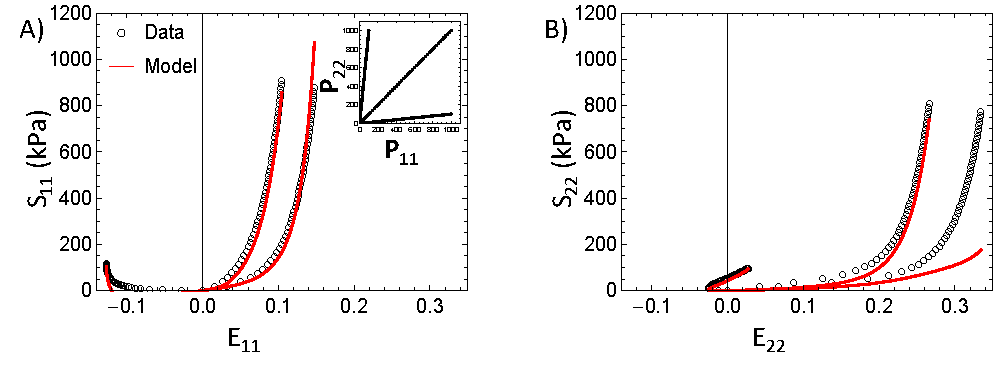
\includegraphics[width=\textwidth]{Images/chapter5/effphypred}
\caption{$\Psi_{eff}$ predicts the A) $S_{11}$ component and B) $S_{22}$ component of the unfitted loading paths very poorly even though the fit to the prestrained range is very good (Fig. \ref{fig:effphyfit}). The inset in A shows the corresponding loading paths.}
\label{fig:effphypred}
\end{figure} 
%-------------------	 end FIGURE 	-------------------%
%%%%%%%%%%%%%%%%%%%%%%%%%%%%%%%%%%%%%%%%%%%%%%%%%%%%%%%%%%%%


	

%%%%%%%%%%%%%%%%%%%%%%%%%%%%%%%%%%%%%%%%%%%%%%%%%%%%%%%%%%%%
%-------------------	begin FIGURE 	-------------------%
\begin{figure}[hptb]
\centering
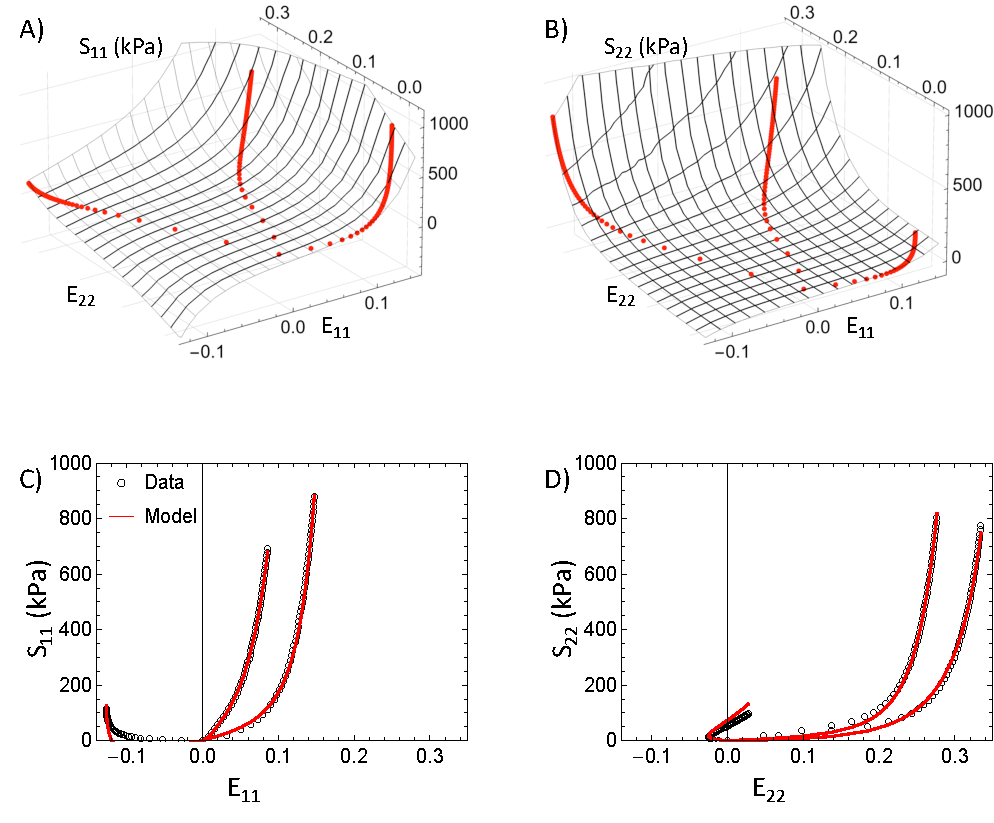
\includegraphics[width=\textwidth]{Images/chapter5/effoptfit}
\caption{$\Psi_{eff}$ fit optimal loading paths very well. A) The $S_{11}$ surface fitted to the data points. B) The $S_{22}$ surface fitted to the data points. C) Best fit of the $S_{11}$ component of the loading paths. D) Best fit of the $S_{22}$ component of the loading paths.}
\label{fig:effoptfit}
\end{figure} 
%-------------------	 end FIGURE 	-------------------%
%%%%%%%%%%%%%%%%%%%%%%%%%%%%%%%%%%%%%%%%%%%%%%%%%%%%%%%%%%%%

%%%%%%%%%%%%%%%%%%%%%%%%%%%%%%%%%%%%%%%%%%%%%%%%%%%%%%%%%%%%
%-------------------	begin FIGURE 	-------------------%
\begin{figure}[hptb]
\centering
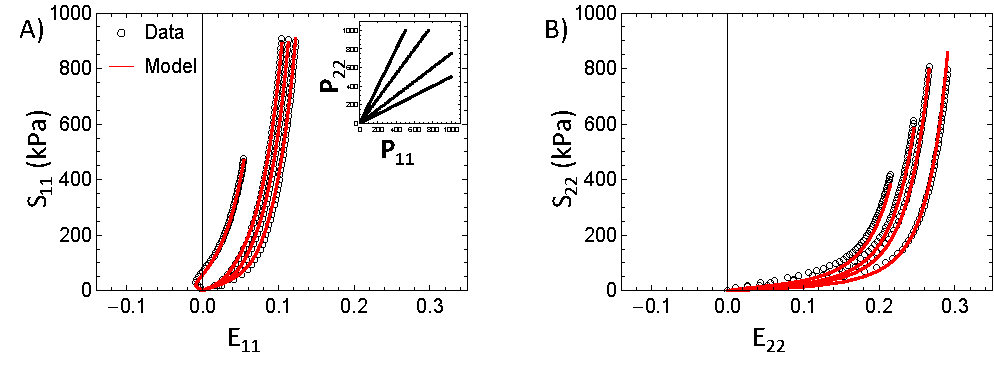
\includegraphics[width=\textwidth]{Images/chapter5/effoptpred}
\caption{Combining $\Psi_{eff}$ with optimal loading paths to predicts the A) $S_{11}$ component and B) $S_{22}$ component of the remaining unfitted loading paths very well from fit (Fig. \ref{fig:effoptfit}). The inset in B shows the corresponding loading predicted paths.}
\label{fig:effoptpred}
\end{figure} 
%-------------------	 end FIGURE 	-------------------%
%%%%%%%%%%%%%%%%%%%%%%%%%%%%%%%%%%%%%%%%%%%%%%%%%%%%%%%%%%%%





	



%%%%%%%%%%%%%%%%%%%%%%%%%%%%%%%%%%%%%%%%%%%%%%%%%%%%%%%%%%%%%
%%  Application to numerical simulations of BHVs under      %
%   quasistatic loading                                     %

\subsection{Numerical simulation of equibiaxial tension process and simulated bioprosthetic heart valve deformation}
	
    Planar biaxial test simulations were conducted to ensure that $\Psi_{eff}$ (Eqn. \ref{eqn:finalexponentialmodelformscaled}) and the elasticity tensor (Appendix \ref{sec:elasticitytensor}, Eqn. \ref{eqn:greenelasticityform}) were properly implemented in the finite element simulation framework.  We compared the computation time for both $\Psi_{eff}$ and Holzapfel-Gasser-Ogden model for biaxial simulation of bioprosthetic heart valve tissues and expectedly found no significant increase in computational cost. The total elapsed time for $\Psi_{eff}$ is 7.58 seconds in comparison to 6.40 seconds for the Holzapfel-Gasser-Ogden model, much faster than any micro-models can achieve.  

	Next we simulated tri-leaflet valves with model parameters derived from bovine pericardium, porcine aortic valve leaflet, and an idealized isotropic case. This is a simple demonstration of the use of the $\Psi_{eff}$ for the upscaling and homogenizing of micro-models. The model parameters for the bovine pericardium case were derived from the simplified structural model and model parameter of Aggarwal and Sacks \cite{aggarwal_inverse_2015}, and the resulting response matched very well qualitatively. Due to a lack of fiber mapping in the quasi-static simulation software used, some minor difference are still expected. We found no difficulty when simulating the pericardium, aortic, or isotropic valves. Suggesting that $\Psi_{eff}$ is quite robust numerically.
	
	
\begin{figure}
\centering
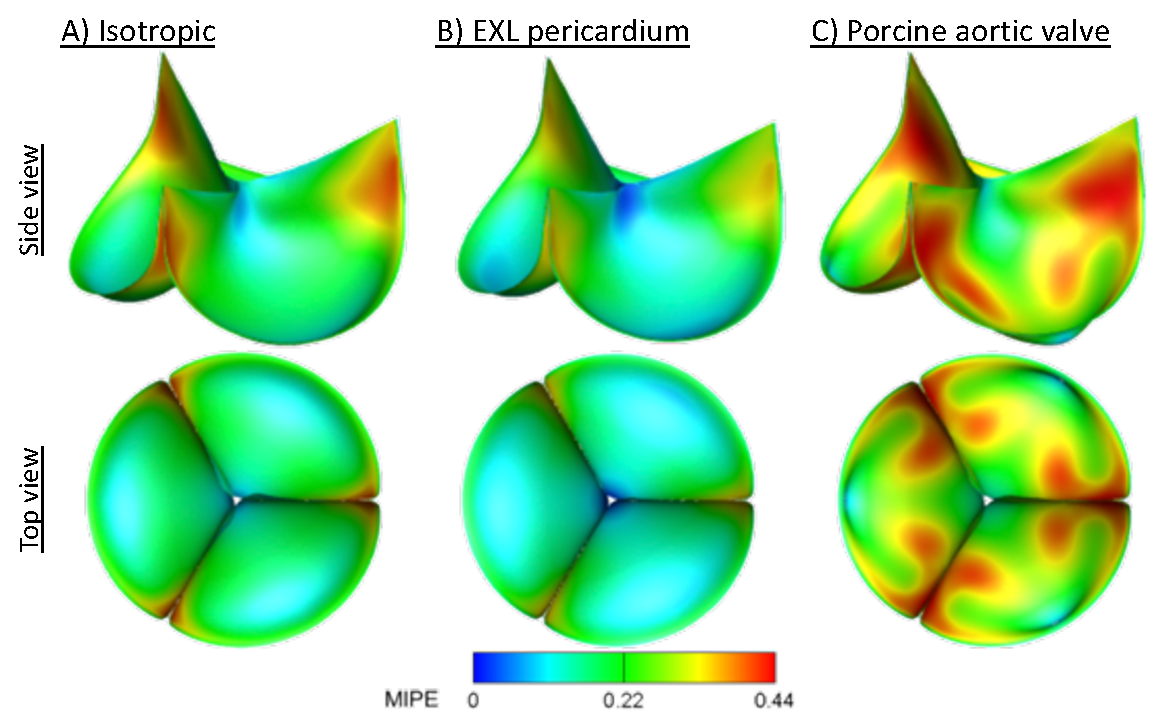
\includegraphics[width=\textwidth]{Images/chapter5/valvesimulations}
\caption{Simulations of intact tri-leaflet valves using A) the porcine aortic valve properties with an uniform fiber orientation distribution, B) exogenously cross-linked bovine pericardium properties with the most homogenous stress distribution, and C) the porcine aortic valve properties properties which results in a very heterogeneous stress distribution and the belly region caving in. The top row shows the side view of the valves at 80 mmHg and the bottom row shows the top-down view of the valves at the same transvalvular pressure.}
\label{fig:valvesimulations}
\end{figure}
    
    The material properties have significant effects on the mechanical behaviors of the leaflets (Fig. \ref{fig:valvesimulations}). The strain distributions within the leaflets were obtained for the pressure-loaded, fully-closed configurations of the valve, and then plotted with the maximum in plane Green-Lagrange strain (MIPE). When comparing the three different material, we can see that the native aortic valve properties result in significant heterogeneities in the deformation of the leaflets (Fig. \ref{fig:valvesimulations}C). Specifically, the belly region of the leaflets significantly protrudes out, increasing the load in the surrounding regions, especially near the commissures. This results in some stress concentrations that are not conducive to heart valve durability and health in general. The bovine pericardium valve (Fig. \ref{fig:valvesimulations}B) and the isotropic valve (Fig. \ref{fig:valvesimulations}A) on the other hand have significantly more homogeneous leaflet deformations, especially from the top-down view. Both of these undergo approximately the same deformation of 0.2 in MIPE. The largest difference between the two is near the commissure regions of the valve. Where the isotropic case is under significantly higher strain. Functionally, the material properties of the exogenously cross-linked bovine pericardium are the most suitable for heart valve leaflets, which distributes the stresses more evenly. 
    
    Much of the reasons behind these differences are likely to be due to the differences between the apparent mechanical properties \textit{in vivo} and the measured mechanical response in the laboratory setting. This is especially true for the aortic valve, which is extremely anisotropic with very high compliance in the radial direction of the leaflets. This difference is most likely due to the mismatch of referential configuration between the two states. Residual strain or residual stress has significant impact on the functional properties of the leaflets, specifically the apparent anisotropy and stiffness. Collagen fiber directions and varying regional properties can also have significant impact on the functional properties of the leaflets, and thus the results of the simulation. The valve leaflet shape, root geometry and properties, the arterial or ventricular geometry and loading conditions, can all be significant factors affecting the functions and stress distribution of the valve leaflets. Furthermore, how these factors affect the fluid dynamics of the valves is also an interesting question, suitable for further study. All in all, this is meant to be a demonstration and proof of concept for using $\Psi_{eff}$ to handle a wide range of soft tissue behaviors and anisotropy for the simulation of biological organs, in this case heart valves. Further and more detailed studies will be reserved for the future.  
  

    
    



%---    Discussion
%%%%%%%%%%%%%%%%%%%%%%%%%%%%%%%%%%%%%%%%%%%%%%%%%%%%%%%%%%%%%
%%	Discussion												%
%%%%%%%%%%%%%%%%%%%%%%%%%%%%%%%%%%%%%%%%%%%%%%%%%%%%%%%%%%%%%

\section{Discussion}

%-----------------------------------------------------------
%	Model performance
%-----------------------------------------------------------
\subsection{Using the effective constitutive model for homogenization in numerical simulations}

	The most fundamental issue with using phenomenological models for soft tissue and organ numerical simulations are that they 1) cannot simulate deformation beyond the range of data used for parameter estimation, and 2) cannot be widely used for tissues other than the ones they are specifically formulated for. Without being able to fully reproduce the response of micro-models, the resulting response may become inconsistent with the mechanisms of these micro-models, impacting their ability to simulate soft tissue responses, particular when modeling time-dependent processes. In the present work we found that using $\Psi_{eff}$ (Eqn. \ref{eqn:finalexponentialmodelformscaled}) along with optimally selected loading paths reconciles this issue. $\Psi_{eff}$ demonstrates much better capabilities at fitting the mechanical response of soft tissues in general. Admittedly, this may not be especially important for simulations of soft tissues in the normal physiological range as most models can fit the response of tissues if the range of deformation is small, as demonstrated with the generalized Fung model. However, for simulating abnormal conditions such as those that will drastically alters the deformation of the tissue, then using $\Psi_{eff}$ will be much more accurate. 
    
    
    The second and equally important part is the need for optimal data to determine the model parameters. Admittedly, the amount of data needed is not necessarily extensive. For example, we have shown that just three carefully selected loading paths can greatly improve the predictive capability of $\Psi_{eff}$ over the entire range of deformations. However, when the loading paths are selected poorly, $\Psi_{eff}$ still has some issue when predicting protocol beyond the range used to fit the model. Examples of this are when only using a single protocol under equi-biaxial stress (Appendix \ref{sec:otherresults}, Fig. \ref{fig:effequifit}D), or only using protocols in the prestrained range (Fig. \ref{fig:effphypred}). Mechanisms are still the major factor limiting the predictive capability in these cases. However, the intended role of $\Psi_{eff}$ is only to homogenize the response of mechanisms-based micro-models, not to help to better understand soft tissue function. The loading paths can be simulated by choice, thus should not be a major factor affecting $\Psi_{eff}$ in numerical simulations. 
    
    
    As we have shown, $\Psi_{eff}$ is able to handle a wide range of soft tissue behavior with no change in model form. This greatly simplifies the need of implementing a different constitutive models for every tissue type, especially when the Jacobian or the elasticity tensor must be implemented separately for computational efficiency, which can be quite complex, i.e. in ABAQUS UMAT. $\Psi_{eff}$ alone is capable of fully reproducing their mechanical response for simulations without significant loss in accuracy. Thus, the use of effective constitutive models can greatly facilitate in not only the computation speed of numerical simulations, but also the speed of implementing constitutive models of different soft tissue for simulations. In these cases, only the parameters of $\Psi_{eff}$ and organ geometry needs to be changed, as we demonstrated for the simulaiton of bovine pericardiu, porcine aortic and isotropic heart valves. $\Psi_{eff}$ is smooth, easily differentiable, and easy to implement. With optimal loading path and model scaling, the process of converting micro-model response to $\Psi_{eff}$ (Eqn. \ref{eqn:finalexponentialmodelformscaled}) should take not more than a few seconds, while saving a significant amount of time during numerical simulations. 
    
    
    On the other hand, micro-models are very useful for reproducing the response of tissue to which the full microstructure are known. This avoids the need for extensive mechanical data and parameter estimation, saving a time consuming step for evaluating different material designs. Some structural and geometry information may also be measurable \textit{in vivo} due to advances in techniques such as 3D ultrasound \cite{steiner_diagnostic_1994, yang_3d_2008, fenster_3_1996} and DT-MRI \cite{basser_vivo_2000, basser_microstructural_2011}, and can be directly incorporated into meso-scale structural models. However, these techniques are not yet sufficient to determine the mechanical properties of tissues. As such, micro-models are still a necessary and important part of any predictive simulation. Not surprisingly, even most traditional invariant based models, such as the Holzapfel-Gasser-Ogden model \cite{holzapfel_new_2000}, are being extended to incorporate the microstructures of the tissue \cite{holzapfel_modelling_2015}. 
    
    

%-------	growth and remodeling	-------%
\subsection{Effective constitutive model applications}

    One application of effective constitutive models is for simulating time-dependent processes, such as growth and remodeling. Growth and remodeling have been a long-time interest of the biomechanics community, and has important role in predictive simulations. Theories for growth and remodeling have been well studied, from Rodriguez in 1994 to Lanir and others in the current time \cite{lanir_mechanistic_2014, gleason_mixture_2004, rodriguez_stress_1994, humphrey_constrained_2002, cowin_tissue_2004, taber_biomechanics_1995}. The general theories for growth and remodeling involve the mechanisms for the changes in the reference configurations and a constrained mixture model involving the combined response of old original materials and new generated materials. This again multiplies the computational cost of the material models and the summation of many individual responses can significantly reduce numerical precision. Here homogenization using $\Psi_{eff}$ (Eqn. \ref{eqn:finalexponentialmodelformscaled}) can be useful. 
    

%-------	inverse modeling	-------%
    Another important application is for inverse modeling, which is important for patient specific modeling. Outside of \textit{in vitro} studies, performing the experiments necessary to determine the mechanical response of soft tissues is extremely difficult. Here, inverse modeling approaches are a solution to this problem \cite{lee_inverse_2014, aggarwal_inverse_2015, aggarwal_patient_2013, kim_inverse_2009, liu_inverse_2013}. In inverse modeling, the model parameters and the errors between the simulated and measured strains are simultaneously optimized. However, the available data that can be obtained \textit{in vivo} is limited, and is not always sufficient to accurately determine the model parameters. In these cases, the tissue microstructure can be used along with meso- and multi-scale models to narrow down the range of possible parameters. However, this multiplies the already hefty costs of the these constitutive models. Here, the approach we proposed (Fig. \ref{fig:simulationframework}B) can be used to reduce computational cost.

 


%-----------------------------------------------------------
%	Model scaling method
%-----------------------------------------------------------

\subsection{Model scaling method in other applications}
    
    Although not introduced as such, the model scaling method, or a similar technique to this, was briefly described by Fung \textit{et al.} in their original work on the mathematical modeling of arteries \cite{fung_pseudoelasticity_1979}. The paper introduced the strain energy density function as 
%==========================================================%
%-------------------	begin EQUATION 	-------------------%
\begin{equation}\label{eqn:fungarterymodel}
\rho_0 W^{(2)} = \frac{C^\prime}{2}\operatorname{exp}\left[\alpha_1 \left(E_{\theta\theta}^2 - E_{\theta\theta}^{*2} \right) + \alpha_2 \left(E_{zz}^2 - E_{zz}^{*2} \right) + \alpha_4 \left(E_{\theta\theta}E_{zz} - E_{\theta\theta}^*E_{zz}^* \right) \right]
\end{equation}
%-------------------	 end EQUATION 	-------------------%
%==========================================================%    
    in equation 2 of the said work ($C$ is changed to $C^\prime$ to consistency in notation with the present work). $E_{\theta\theta}^*$ and $E_{zz}^*$ are introduced as strains corresponding to some fixed stresses of $S_{\theta\theta}^*$ and $S_{zz}^*$, usually taken in the physiologic range. Similarly, this "scaling" can be absorbed into the parameter $C^\prime$ like in the present work. This idea was not greatly expanded upon, but \textit{Fung et al.} notes that:
\begin{quotation}
"But in practice it is very helpful to introduce $E_{\theta\theta}^*$ and $E_{zz}^*$. Not only are the values corresponding to $S_{\theta\theta}^*$ and $S_{zz}^*$ very important information, but also their use makes the constants [$C^\prime$], $\alpha_1$, $\alpha_2$, and $\alpha_4$ much more stable for each set of specimen." \cite{fung_pseudoelasticity_1979}
\end{quotation} 
    and that 
\begin{quotation}
"[$E_{\theta\theta}^*$ and $E_{zz}^*$] are indexes of compliance of the vessel. Using $E_{\theta\theta}^*$ and $E_{zz}^*$, the variations of the constants $C$, $\alpha_1$, $\alpha_2$, and $\alpha_4$, which determines the shape of the stress-strain curve, are greatly reduced. The assignment of $S_{\theta\theta}^*$ and $S_{zz}^*$ is arbitrary, but hopefully standard values will be adopted by the biomechanics community." \cite{fung_pseudoelasticity_1979}
\end{quotation}

	In truth, we did not find that the model scaling method necessarily makes $\alpha_1$, $\alpha_2$, and $\alpha_4$ more consistent, but rather that they are exactly the same values with or without this method, assuming parameter estimation was not trapped in some local minimum. The model scaling method does make reaching the values of these parameter more consistent. The biggest benefit remains the significant improvement in the correlation between the parameters $C^\prime$ and $\alpha_1$, $\alpha_2$, and $\alpha_4$, improving the conditioning of the objective function surface during parameter estimation. It also imparts some physical meaning to the value of $C^\prime$, or for $A_s$ and $c_0^\prime$ in present work. For Fung \textit{et al.}, this is some arbitrary physiologic stresses, for us, this is exactly 'maximum' (with respect to the objective function) value of strain energy within the data used for parameter estimation. This does bestow some consistency to the value of $C^\prime$, as it is exactly the total strain energy density at the stresses of $S_{\theta\theta}^*$ and $S_{zz}^*$, which will likely be similar between specimens taken from the same arteries from health subjects. However, the choice of $E_{\theta\theta}^*$ and $E_{zz}^*$, or $E_m^\mathrm{max}$, $E_n^\mathrm{max}$, and $E_\phi^\mathrm{max}$ for $\Psi_{eff}$ (Eqn. \ref{eqn:finalexponentialmodelformscaled}), should not be arbitrary. The model scaling method works due to altering the functional effect of $c_0$ and $b_i$, or $C$ and $\alpha$. $E_m^\mathrm{max}$, $E_n^\mathrm{max}$, and $E_\phi^\mathrm{max}$ should be chosen deliberately so that area under the constitutive model, based on the objective function, remains approximately the same, thus decoupling changes in modulus and changes in curvature from the exponential parameters. 


	Perhaps, the biggest advantage of the model scaling method is that it is applicable to nearly any constitutive model with an exponential function, such as models like the Holzapfel-Gasser-Ogden, Humphrey, Vito, or even the meso-scale structural model with simplified ensemble response such as in Fan and Sacks \cite{fan_simulation_2014a}, Lee \textit{et al.}\cite{lee_effects_2015}, and Aggarwal and Sacks \cite{aggarwal_inverse_2015}. Even polynomial model forms with a power law, $\Psi=A\epsilon^B$, such as the generalized Ogden model, or the elastin model for the mitral valve in Zhang et al. \cite{zhang_meso_2016} can see benefits from the model scaling method. In this case, the scaling term becomes $A = \bar{A} e^{-B \log(\epsilon_{max})}$. In summary, this model scaling method should have significantly implications in improving the speed and consistency of parameter estimation for any model with an exponential like form.
    
    
    
    
%-----------------------------------------------------------
%	Optimal
%-----------------------------------------------------------	
\subsection{The equibiaxial stress protocol in optimal loading paths}

    One highlight from the optimal loading path study is that the equibiaxial stress loading path is extremely important. The equibiaxial stress loading path is always the one shown in figures for most paper, as it gives most intuitively understandable information on the mechanical properties of the tissue. It gives insights into the general form, anisotropy and stiffness of the material at a glance, and is not surprisingly also the best loading path for parameter estimation. However, it is surprising just how little the equibiaxial stress loading path can provide alone. The difference in magnitude between the D-optimality values for one vs. two loading paths is almost 20. The equibiaxial stress alone simply is not enough to determine the material parameters using phenomenological approaches. However, with the addition of one or two more protocols, even if they are along a similar loading paths can significantly improve the predictive capabilities. However, this may be partially overcome by meso-scale structural approaches, given the information on the microstructure of the tissue.


\subsection{Alternative options for optimal \textit{in silico} loading paths}

	The limitation on predicting outside of the loading paths used for parameter estimation can be somewhat remedied by densely sampling the response of the micro-model over a larger range of deformations. However, this is not entirely ideal for computational speed during parameter estimation, and choosing the sampling points for parameter estimation is not a trivial task itself. Points with high stresses tend to weight heavily during parameter estimation, proper care needs to be taken to capture both the high stress and low stress response. Given that the number of data points scales cubically with the distance between data points, this approach is still limited. 

    
    Having said this, our investigation of optimal loading paths is restricted to constant strain ratios or constant stress ratios. In reality, there are many ways to define loading paths, some can be quite creative. We do not deny the possibility of other forms of loading paths that are more optimal. However, the current approach with three, or at most five protocols, is already sufficient. We did test some alternative loading paths, such as Fung \textit{et al.}'s post pre-strain loading paths \cite{fung_pseudoelasticity_1979}. They cover much of the physiological range, but are still insufficient for parameter estimation. Increasing the number of loading paths in this case has minor improvements, but pales in comparison to just picking better types of loading paths. The poor predictive capabilities for the low stress region can have significant impacts on underestimating the mechanical properties of matrix and elastin, and their properties can be important to the functions of micro-models. The mechanical properties of the matrix for example, having significant implications for simulating the process of permanent set in exogenously cross-linked soft tissues \cite{zhang_modeling_2017}. Failing to properly reproduce this response, can affect the predictive capabilities of the associated micro-models, causing the whole framework of using $\Psi_{eff}$ to facilitate numerical simulations (Fig. \ref{fig:simulationframework}B) to fall apart. 
    
    










%---    Conclusion
%%%%%%%%%%%%%%%%%%%%%%%%%%%%%%%%%%%%%%%%%%%%%%%%%%%%%%%%%%%%%
%%	Conclusion												%
%%%%%%%%%%%%%%%%%%%%%%%%%%%%%%%%%%%%%%%%%%%%%%%%%%%%%%%%%%%%%

% \section{Limitations and conclusion}

%-----------------------------------------------------------
%	Limitations
%-----------------------------------------------------------
\section{Limitations} 
	
    One major limitation of $\Psi_{eff}$ (Eqn. \ref{eqn:finalexponentialmodelformscaled}) is the large number of parameters, 14 in the fully generalized form. This is not very favorable, as the time complexity for most optimization algorithms scales nonlinearly with the number of parameters. However, $\Psi_{eff}$ has very low computational cost, and reasonably low parameter covariance, thus this should not be a major problem. Alternatives are also less favorable, as they either require more parameters or cannot sufficiently capture the response of soft tissues in a wide range or reproduce the response of multiple tissue types. 
    
    Another limitation, which also applies to all phenomenological models, is that $\Psi_{eff}$ has no intrinsic mechanisms built in. Without sufficient mechanical data to derive the model parameters, phenomenological models have limited predictive capabilities. Specifically, the phenomenological models perform poorly when extrapolating outside of the range of available data. This also means that phenomenological models can only provide limited information on how the tissue functions. It can reproduce the mechanical response of soft tissues very well, but it is also harder to infer more about the structure and function of the tissue. This is not a major concern for us. For the mechanisms or the structure to function relationship of soft tissues, micro-models already fulfills the need. $\Psi_{eff}$ is intended as a fit all model for fulfilling the gap between predictive micro-models and computationally efficient simulations. With carefully selected of loading paths for parameter estimation (Section \ref{sec:optimaldesign}), $\Psi_{eff}$ can accurately reproduce the mechanical response of soft tissue within the expected range. In other words, $\Psi_{eff}$ does not have to be able to predict the mechanical response of soft tissues under unmeasured and extrapolated deformations, it only has to be able to fully reproduce the entire range of responses predicted by the micro-models, which is its main purpose. 



%-----------------------------------------------------------
%	Conclusion
%-----------------------------------------------------------
\section{Conclusion and Future Directions} 

	In this work, we developed a constitutive model form for the effective response of planar soft tissues. This effective constitutive model (Eqn. \ref{eqn:finalexponentialmodelformscaled}) is applicable to a wide range of soft tissue responses, while being as computationally efficient as most common phenomenological approaches, such as Holzapfel-Gasser-Ogden or the generalized Fung model. This model utilizes the modeling scaling method for minimizing covariance between parameter, which shows significant improvements in the speed and accuracy of parameter estimation. We have shown that our effective constitutive model along with optimal loading paths is able to fully replicate the response of complex meso-scale structural models for the entire range of deformations, whereas most phenomenological models have difficulties when predicting unfitted loading paths. The effective constitutive model is robust enough to be able to handle a wide range of soft tissue behaviors and anisotropy for accurate numerical simulations, such as in simulations of heart valves. Thus, the effective constitutive model can play an important role for the upscaling and homogenization of the response of complex micro-models for improving the efficiency of organ-level simulations. 
    

	One nature extension to this effective modeling approach is for 3 dimensional soft tissues. The extension to 3 dimensions doubles the number of inputs in comparison to planar models, with the additional inputs being $E_{13}$, $E_{23}$, and $E_{33}$. This means that the initial most generalized form for the 3-D soft tissue models (Eqn. \ref{eqn:exponentialmodelform}) has 209 terms before reduction. This is unmanageable for establishing the initial approach, where using a planar soft tissue model is more suitable. However, applying the same restrictions to the model form (section \ref{sec:finalform}) reduces this to 48 terms. This is possible due to symmetry by expressing the components of the Green-Lagrange strain tensor with respect to the material axis (Eqn. \ref{eqn:greenstrain}). This is not so easy to do in 3-dimensions, requiring a third vector corresponding to the direction of least stiffness, which in turn requires the 3 dimensional fiber orientation distribution. 
    
    
    
    
    
    
    
    





%---    Bioliography
\bibliographystyle{plainnat}
\bibliography{phd}